%% Version 4.3.2, 25 August 2014
%
%%%%%%%%%%%%%%%%%%%%%%%%%%%%%%%%%%%%%%%%%%%%%%%%%%%%%%%%%%%%%%%%%%%%%%
% Template.tex --  LaTeX-based template for submissions to the 
% American Meteorological Society
%
% Template developed by Amy Hendrickson, 2013, TeXnology Inc., 
% amyh@texnology.com, http://www.texnology.com
% following earlier work by Brian Papa, American Meteorological Society
%
% Email questions to latex@ametsoc.org.
%
%%%%%%%%%%%%%%%%%%%%%%%%%%%%%%%%%%%%%%%%%%%%%%%%%%%%%%%%%%%%%%%%%%%%%
% PREAMBLE
%%%%%%%%%%%%%%%%%%%%%%%%%%%%%%%%%%%%%%%%%%%%%%%%%%%%%%%%%%%%%%%%%%%%%

%% Start with one of the following:
% DOUBLE-SPACED VERSION FOR SUBMISSION TO THE AMS
\documentclass{ametsoc}

% TWO-COLUMN JOURNAL PAGE LAYOUT---FOR AUTHOR USE ONLY
% \documentclass[twocol]{ametsoc}

%%%%%%%%%%%%%%%%%%%%%%%%%%%%%%%%
%%% To be entered only if twocol option is used

\journal{jcli}

%  Please choose a journal abbreviation to use above from the following list:
% 
%   jamc     (Journal of Applied Meteorology and Climatology)
%   jtech     (Journal of Atmospheric and Oceanic Technology)
%   jhm      (Journal of Hydrometeorology)
%   jpo     (Journal of Physical Oceanography)
%   jas      (Journal of Atmospheric Sciences)	
%   jcli      (Journal of Climate)
%   mwr      (Monthly Weather Review)
%   wcas      (Weather, Climate, and Society)
%   waf       (Weather and Forecasting)
%   bams (Bulletin of the American Meteorological Society)
%   ei    (Earth Interactions)

%%%%%%%%%%%%%%%%%%%%%%%%%%%%%%%%
%Citations should be of the form ``author year''  not ``author, year''
\bibpunct{(}{)}{;}{a}{}{,}
\usepackage[super]{nth} %adds superscripts for things like 20th

%%%%%%%%%%%%%%%%%%%%%%%%%%%%%%%%

%%% To be entered by author:

%% May use \\ to break lines in title:

\title{Climatology and Decadal Change of Rainbands over China: The Rainband Detection Algorithm (RDA)}

%%% Enter authors' names, as you see in this example:
%%% Use \correspondingauthor{} and \thanks{Current Affiliation:...}
%%% immediately following the appropriate author.
%%%
%%% Note that the \correspondingauthor{} command is NECESSARY.
%%% The \thanks{} commands are OPTIONAL.

    %\authors{Author One\correspondingauthor{Author One, 
    % American Meteorological Society, 
    % 45 Beacon St., Boston, MA 02108.}
% and Author Two\thanks{Current affiliation: American Meteorological Society, 
    % 45 Beacon St., Boston, MA 02108.}}

\authors{Jesse A. Day\correspondingauthor{Jesse Day, University of California, Department of Earth and Planetary Science, College of Letters and Science, 307 McCone Hall, Berkeley, CA 94720.}, Inez Y. Fung and Weihan Liu}

%% Follow this form:
    % \affiliation{American Meteorological Society, 
    % Boston, Massachusetts.}

\affiliation{Department of Earth and Planetary Science, University of California Berkeley, Berkeley, California}

%% Follow this form:
    %\email{latex@ametsoc.org}

\email{jessed@berkeley.edu}

%% If appropriate, add additional authors, different affiliations:
    %\extraauthor{Extra Author}
    %\extraaffil{Affiliation, City, State/Province, Country}

%\extraauthor{}
%\extraaffil{}

%% May repeat for a additional authors/affiliations:

%\extraauthor{}
%\extraaffil{}

%%%%%%%%%%%%%%%%%%%%%%%%%%%%%%%%%%%%%%%%%%%%%%%%%%%%%%%%%%%%%%%%%%%%%
% ABSTRACT
%
% Enter your abstract here
% Abstracts should not exceed 250 words in length!
%
% For BAMS authors only: If your article requires a Capsule Summary, please place the capsule text at the end of your abstract
% and identify it as the capsule. Example: This is the end of the abstract. (Capsule Summary) This is the capsule summary. 

\abstract{The topography and continental configuration of East Asia favor the year-round existence of zonal storm tracks that extend thousands of miles from eastern China into the northwestern Pacific Ocean. During a period known as Meiyu season (late spring and early summer), intense rainfall along these tracks (the ``Meiyu Front'') contributes the bulk of East Asian summer monsoon seasonal totals. While individual frontal events have been studied by Chinese meteorologists for decades, no multi-decadal statistical characterization exists. We present a novel image processing algorithm, the Rainband Detection Algorithm (RDA), that can detect rainbands in maps of daily rainfall and quantify their attributes. By applying RDA to the APHRODITE database of Asian monsoon rainfall over the region 105$^{\circ}$-123$^{\circ}$E and 20$^{\circ}$-40$^{\circ}$N, we produce a 57-year (1951-2007) daily catalog of all rainband occurrences over China (20,819 days total). Rainfall on each individual day is also partitioned into banded and ``local'' (non-banded) components, each reflecting different mechanisms of rainfall. The seasonal progression of the East Asian monsoon and Meiyu Front are quantified as a series of jumps in the frequency and intensity of rainbands. Furthermore, it is found that the ``South Flood-North Drought'' tendency of late \nth{20} century rainfall, described previously in other studies, corresponds primarily to changes in the frequency of banded rainfall.}
\begin{document}

%% Necessary!
\maketitle


%%%%%%%%%%%%%%%%%%%%%%%%%%%%%%%%%%%%%%%%%%%%%%%%%%%%%%%%%%%%%%%%%%%%%
% MAIN BODY OF PAPER
%%%%%%%%%%%%%%%%%%%%%%%%%%%%%%%%%%%%%%%%%%%%%%%%%%%%%%%%%%%%%%%%%%%%%
%

%% In all cases, if there is only one entry of this type within
%% the higher level heading, use the star form: 
%%
% \section{Section title}
% \subsection*{subsection}
% text...
% \section{Section title}

%vs

% \section{Section title}
% \subsection{subsection one}
% text...
% \subsection{subsection two}
% \section{Section title}

%%%



\section{Introduction} 

 	Eastern China receives about 60\% of its precipitation from May to August via the East Asian summer monsoon. The period of peak rainfall lasting from early June to mid-July is called ``Meiyu season'' (lit. ``plum rains,'' referring to the spectacular growth of plum blossoms in central China with the onset of heavy rains). During this time, heavy rainfall occurs in zonal bands resulting from frontal synoptic conditions (the ``Meiyu Front''). The rainfall climatology of Japan and Korea also features similar phenomena, known as Baiu and Changma respectively, that deliver key fractions of total yearly rainfall. While banded rainfall is known to contribute a significant component of yearly totals across East Asia, its role has not been quantified across a large sample of days.
	
		The climatology of the East Asian monsoon is unique when compared to other monsoon circulations \citep{Ding2005}. Whereas understanding of tropical monsoons has progressed greatly via theoretical studies \citep{Plumb1992,Prive2007,Bordoni2008}, the dynamics that favor the existence of frontal convection over East Asia in summer remain a point of debate, centering around the interplay of the tropospheric jet and Tibetan Plateau \citep{Molnar2010,Sampe2010,Chen2014}. It is known that the migration of the Meiyu front entails a series of large-scale circulation changes \citep{Chen2004}, and furthermore that anomalies in Meiyu front latitude produce corresponding rainfall anomalies \citep{Kosaka2011}. 
		
	We have developed a recursive image processing algorithm, the Rainband Detection Algorithm (RDA), which locates frontal rainbands in a daily precipitation map and quantifies their attributes. By applying this algorithm to the APHRODITE historical record of Asian monsoon rainfall, we have created a 57-year (1951-2007) daily database of rainband attributes in China. Previous studies have investigated the statistics of the Meiyu front on decadal and even centennial timescales \citep{Chen2004,Ge2008,Xu2009}, but to our knowledge no previous author has compiled a multi-decadal daily catalog of events. 
		
	This paper presents the RDA algorithm and a China rainband catalog. We display the seasonal progression of the East Asian monsoon and the Meiyu Front in unprecedented fashion by partitioning daily rainfall into two components: Banded rainfall (extending zonally at least 500 km) and local storms. We argue that this classification reflects different mechanisms of formation. In \citep{Day2015}, we showed that the length scale of storms across the entire Asian monsoon tends to be about 200-300 km. In contrast, although RDA uses a cutoff of 500 km as minimum rainband length, mean yearly rainband length is about 1200 km (Figure~\ref{hov}). Local storms can occur due to anomalous self-buoyancy or orographic triggering, while banded rainfall likely reflects the existence of larger-scale convergence or frontal conditions.  We cannot rule out that other mechanisms of rainfall are capable of forming rainbands, but China demonstrates unusual zonal coherence, reflecting a consistent mechanism of genesis. As shown subsequently, banded and local rainfall display distinct seasonal cycles, suggesting that their origins are separate.
	
%Hadn't really considered this previously, but these frontal storms are both a response to large-scale, but also alter synoptic environment and play a climatological role in setting patterns of diabatic ascent and descent. A response and forcing - see Newman et al. 2016, where individual storms in Pacific effect heat transport. Also O'Reilly and Czaja 2015
	
\section{Data Sets}

	The APHRO\_MA\_V1101 product from APHRODITE (Asian Precipitation - Highly-Resolved Observational Data Integration Towards Evaluation of the Water Resources) includes 57 years (1951-2007) of continental daily rainfall (PRECIP product) on a .25$^{\circ} \times .25^{\circ}$ grid over 60$^{\circ}$-150$^{\circ}$E and 15$^{\circ}$S-55$^{\circ}$N \citep{Yatagai2012}, as well as a daily map of available weather stations on the same grid (RSTN product). Values are assimilated from weather station observations and therefore available over land only. We focus on the subregion inside of 105$^{\circ}$E-123$^{\circ}$E and 20$^{\circ}$N-40$^{\circ}$N, where rainbands are known to occur frequently, especially during Meiyu season. Stations in this region are spaced at 100-200 km intervals, such that rainbands are clearly resolved. APHRODITE's resolution cannot capture some features visible in TRMM satellite data \citet{Xu2009}, but its length allows for the study of decadal change. Since almost all precipitation in this region falls as rain, we use the words ``rainfall'' and ``precipitation'' interchangeably in the rest of this work.
	
\section{Rainband Detection Algorithm (RDA) Functionality}

\subsection{Overview}

	For each day from 1 January 1951 to 31 December 2007 (20,819 days total), RDA determines whether a rainband exists inside the window of 105-123$^{\circ}$E and 20-40$^{\circ}$N, a region hereafter referred to as ``East China.'' A rainband is defined as a continuous chain of rainfall maxima exceeding 10 mm day$^{-1}$ spanning at least 5$^{\circ}$ of longitude. If a rainband exists, its properties are calculated including latitude, intensity, tilt, length and width, as well as a ``quality score'' $Q$, defined as the fraction of daily total East China rainfall falling within the band. Fits with poor $Q$ are not classified as bands. We also test for the existence of two rainbands on a single day, an arrangement commonly found in August and September. In such a case, the first and second fitted rainbands are referred to as ``primary'' and ``secondary'' rainbands respectively. A description of algorithm functionality in greater detail follows.
	
	We cannot distinguish between the mechanisms that supply rainfall. Any storm that propagates zonally over the course of a day will be interpreted as a rainband, regardless even of whether it propagates westward or eastward. However, from observation, storms reaching East China during the rainiest months of the East Asian summer monsoon are predominantly westerly \citep{Day2015}. Therefore, we expect that RDA detects similar types of rainfall events from one summer to the next, allowing for meaningful analysis of decadal changes.  
	
\subsection{Recursive Convergent Image Processing}

\begin{enumerate}
	\item Given a daily map of East China rainfall (105-123$^{\circ}$E, 20-40$^{\circ}$N) at $.25^{\circ} \times .25^{\circ}$ resolution, the maximum rainfall intensity $int_{max}$ and its latitude $lat_{max}$ are recorded at each longitude. If there exists a continuous chain of maxima spanning $5^{\circ}$ of longitude (20 points in a row) where $int_{max}$ exceeds 10 mm day$^{-1}$, we proceed to step 2 and attempt a rainband fit (Figure~\ref{fig:f32}a). Otherwise, there is no rainband and no fit is attempted for that day (Figure~\ref{fig:f32}b).
	
	\item A weighted least-squares linear regression of $lat_{max}$ using $int_{max}$ as weighting approximates the position of the rainband with a straight line (a reasonable assumption from observation). To encourage convergence, the weight of outlying maxima is set to zero. An outlier is defined as any maximum where $lat_{max}$ is over $5^{\circ}$ of latitude away from  $\left<lat_{max}\right>$, the centroid of $lat_{max}$ weighted by $int_{max}$\footnote{In rare cases with two rainbands of roughly equal strength that are well-separated in latitude, the centroid of precipitation may lie midway between the bands such that all maxima will be thrown out as outliers. To avoid this scenario, we verify after removing outliers that

%% FOOTNOTE
	\begin{equation*}
	 \sum\limits_{long} weights > 200 \mathrm{\ mm\ day}^{-1}
	\end{equation*}
	
 	When this condition is failed, which can only occur when too many of our maxima have been discarded, we return to step 1 and find maxima inside a subwindow with latitude range of 20$^{\circ}$N-$\left<lat_{max}\right>$ or $\left<lat_{max}\right>$-40$^{\circ}$N, depending on which half of our domain has a longer chain of maxima exceeding 10 mm day$^{-1}$. The remaining steps of our algorithm are applied as usual. The search for a secondary rainband and calculation of quality scores are performed over the whole East China window (20$^{\circ}$N-40$^{\circ}$N).}, calculated as %%END FOOTNOTE

	\begin{equation*}
	\left<lat_{max}\right>=\frac{\sum_{long} lat_{max}*int_{max}}{\sum_{long} int_{\max}}
	\end{equation*}

	\item A recursive algorithm converges from this initial fit to a best estimate of rainband position. In each iteration, we find a new set of maxima within \textit{k} degrees of the previous best fit line, and again perform a weighted linear fit of the maxima (Figure~\ref{fig:f33}a). $k$ is progressively decreased with each iteration from $5^{\circ}$ to $2^{\circ}$ by $.25^{\circ}$ increments, and then from $2^{\circ}$ to $.25^{\circ}$ by $.25^{\circ}$ increments repeating each width $k$ twice in a row (Figures~\ref{fig:f33}b-c). The fit obtained in the final iteration is taken as our best estimate (Figure~\ref{fig:f33}d).
	
	\item We define the ``quality score'' $Q$ as the fraction of daily total East China rainfall (the sum of all rainfall inside of 105-123$^{\circ}$E and 20-40$^{\circ}$N) that falls within $2.5^{\circ}$ degrees of the best estimate line (Figure~\ref{fig:f34}b). Other rainband properties are calculated as follows:
	
	 \begin{enumerate}
	 
	 	\item \textit{Latitude}: The latitude of the best fit line at 115$^{\circ}$E. 
	 
	 	\item \textit{Intensity}: Mean rainfall of all ``rainband points'' (points along the best fit line where daily rainfall exceeds 5 mm day$^{-1}$).
	 
	 	\item \textit{Length}: Total number of rainband points (units of degrees longitude)
	 
	 	\item \textit{Width}: Mean distance between half-maxima ($int_{max}$/2) on either side of each rainband point (units of degrees latitude).
	 
	 \end{enumerate}
	
	\item After finding a primary rainband, we check for the existence of a secondary rainband by removing all \textit{banded rainfall} associated with the primary band from the daily rainfall map. \textit{Banded rainfall} is defined as all rainfall falling within 4$^{\circ}$ of a rainband axis and any other adjacent points where rainfall exceeds 10 mm day$^{-1}$ (see Figure~\ref{fig:f35}a for an example). After removing primary rainband rainfall, we reapply the continuous maximum criterion from step 1 (Figure~\ref{fig:f35}b). If passed, steps 2-4 are repeated to find a best estimate for the position of the secondary rainband, and its attributes calculated.
	
	\item If a secondary rainband is found, two additional \textit{conditional} quality scores $Q_1$ and $Q_2$ are calculated. $Q_1$ is the fraction of total daily East China rainfall that fell within $2.5^{\circ}$ degrees of the primary rainband \textit{after removing all rainfall associated with the secondary rainband} (effectively the $Q$ score if the secondary rainband didn't exist). Likewise, $Q_2$ is the $Q$ score of the second rainband \textit{after removing all rainfall from the primary rainband}. An example is shown in Figure~\ref{fig:f34}d.		
	
\end{enumerate} 

\subsection{Quality Control}

	After running the algorithm for all 20,819 days from 1 January 1951 to 31 December 2007, we obtained 11,228 days with at least one rainband and 1,116 days with two rainbands. Subsequently, we apply a quality control (QC) algorithm to eliminate days with poor fit, based on the quality scores $Q$, $Q_1$ and $Q_2$ as well as the ``Taiwan fraction'' $TW$, defined as the percentage of daily total East China rainfall falling over the island of Taiwan (roughly 120-$122^{\circ}$E and 22-$26^{\circ}$N). Rainband fits are deemed successful if they satisfy the following two criteria:

\begin{enumerate}

	\item $TW < 20\%$. If $TW > 20\%$, the day's fit is thrown out (238 cases total, 2.1\% of total fits). Such days are dominated by tropical storms reaching Taiwan and do not exhibit a strong rainband (example shown in Figure~\ref{fig:f34}a).  
	
	\item The quality scores of the fit must meet either of the two following benchmarks:
	
	\begin{enumerate} 
	
	\item If $Q>.6$, the fit is deemed successful (7,522 days, 67.0\% of total fits; Figure~\ref{fig:f34}b). If $Q_2$ is also greater than .6, the day will be classified as a double rainband day (Type I double rainband; 232 cases). 3.1\% of days where $Q>.6$ also achieve $Q_2>.6$.
		
	\item If $Q<.6$, the fit is discarded unless two rainbands are detected and both $Q_1 > .6\mathrm{\ \textbf{and}\ }Q_2 > .6$ (where again $Q_1$ and $Q_2$ are \textit{conditional} quality scores as defined above). In such cases, the presence of multiple rainbands of similar intensity initially obscures the goodness of fit (Figure~\ref{fig:f34}d). Such days are also classified as double rainband days (Type II double rainband; 466 cases).
	
	\end{enumerate}
	
	If neither criterion 2a nor 2b is satisfied, the fit is thrown out (Figure~\ref{fig:f34}c).
	
\end{enumerate}	

	The use of conditional quality scores $Q_1$ and $Q_2$ adds 466 double rainband fits (6.2\% of all successful fits) that would otherwise have been missed due to $Q<.6$. 33.2\% of double rainband days are Type I ($Q>.6$) and 66.8\% Type II ($Q<.6$) as defined above. Double rainbands are more common during certain months, particularly July-September. Tables~\ref{tab:t31}-~\ref{tab:t33} contain detailed results of the application of RDA to years 1951-2007 in APHRODITE. The entire catalog is publicly available on the author's website.

\subsection{Rainfall Types}
	
	RDA allows us to classify all rainfall on each day as either \textit{banded} (falls within a rainband) or \textit{local}. \textit{Banded} rainfall consists of all rainfall falling within 4$^{\circ}$ of a rainband axis and any other adjacent points where rainfall exceeds 10 mm day$^{-1}$, the same definition as in step 5 of the recursive algorithm above. An example is shown in Figure~\ref{fig:f35}a. Rainfall on each of the 20,819 available days was partitioned into its banded and local components. This allows us to determine what fraction of rainfall at each point in East China is supplied via banded rainfall (Figure~\ref{fig:frontpct}). We also test for the significance of decadal changes in banded and local rainfall separately (Figure~\ref{fig:type_decadal}). These results are discussed below. Videos of the climatological progression of banded and local rainfall are available at the author's website and on request, as well as daily maps of banded and local rainfall for the years 1951-2007.
	
\section{Methods}	

\subsection{Alternative Metrics of China Rainfall}

Since the RDA method is complex, we must justify its use by proving that it supplies information about China rainfall beyond what simpler metrics can provide. We define a suite of potential daily rainfall metrics as follows: 

\begin{itemize}

	\item $M_1$ - Latitude of maximum rainfall;
	
	\item $M_2$ - Intensity-weighted centroid of daily rainfall latitude;
	
	\item $M_3$ - Intensity of maximum rainfall over China (100-123$^{\circ}$E and 20-40$^{\circ}$N);
	
	\item $M_4$ - Area-averaged intensity of China rainfall; 
	
	\item $M_5$ - Area-averaged intensity of North China rainfall (107.5-125$^{\circ}$E and 37-42$^{\circ}$N); 
	
	\item $M_6$ - Area-averaged intensity of South China rainfall (107.5-122.5$^{\circ}$E and 27-33$^{\circ}$N); 
	
	\item $M_7$ - \% of days where $M_5$ exceeds 1 mm day$^{-1}$ (\textit{frequency} of North China rainfall);
	
	\item $M_8$ - \% of days where $M_6$ exceeds 1 mm day$^{-1}$ (\textit{frequency} of South China rainfall).
	
\end{itemize}

 The definitions of the North China and South China regions are the same as in \citet{Yu2010}. A seasonal climatology of each metric is presented in Figure~\ref{fig:met_climo}, and mean values during different seasons listed in Tables~\ref{tab:t35} and \ref{tab:t36} for the periods 1951-1979 and 1980-2007, with significant changes between the two time periods demarcated.
 
%
%\subsection{Temporal Autocorrelation}
%
%	Fronts and rainbands tend to persist for several days. Therefore, rainfall amounts and front attributes on successive days are not fully independent observations, which reduces the effective number of degrees of freedom of these time series. This temporal autocorrelation must be accounted for in calculations of statistical significance such as estimating the $p$-value of a change in rainband frequency between two time periods. In this particular case, we use the analytic formula for a Bernoulli process (applicable for any time series where observations are binary) with effective number of degrees of freedom $n=\frac{N}{\tau}$ for number of days $N$ and decorrelation time $\tau$ given by
%
%\begin{equation*}
%\tau=1+2\sum_{k=1}^m \rho(k)
%\end{equation*}
%
%	where $\rho(k)$ is the autocorrelation function of rainband existence with lag $k$ \citep{VonStorch1999}. We calculate $\tau$ using a maximum lag of $m=10$ days. The yearly mean decorrelation timescale of rainband frequency is found to be $\tau = 1.81$ after removing the seasonal cycle. This value is used to calculate significance of changes in Figure 3b. The standard deviation and $p$-values of rainband frequency changes in Tables~\ref{tab:t35} and~\ref{tab:t37} use seasonal values of $\tau$ calculated in \ref{tab:t34}. Similarly, Table~\ref{tab:t311} shows the $\tau$ of alternative metrics of China rainfall, which is then used to calculate the significance of decadal changes in Table~\ref{tab:t312}. $\tau$ is also used to select block length for moving blocks bootstrap tests, as described below.

\section{Results}

\subsection{Rainband Climatology}

	We compile our daily rainband catalog into a 57-year daily climatology (1951-2007). Abrupt climatological shifts occur simultaneously in both rainfall and rainband climatology. We define 5 periods of distinct behavior as demarcated in Figure~\ref{fig:hov}, with the Pre-Meiyu, Meiyu and Post-Meiyu equivalent to the three stages of Meiyu rainfall described in \citet{Ding2005}.

\begin{enumerate}

\item The Spring Rains (days 60-120, March 1-April 30), previously studied in \citet{Tian1998}, marked by frequent but relatively weak rainbands (47\% occurrence, 20 mm day$^{-1}$ mean);

\item Pre-Meiyu season (days 121-160, May 1-June 9), during which rainfall and front intensity steadily increase (56\% occurrence, 25.5 mm day$^{-1}$ mean);

\item Meiyu season (days 161-200, June 10-July 19) when a remarkable 7-degree northward shift in mean rainband latitude occurs over the course of several weeks, and rainband frequency and intensity peaks (66\% occurrence, 28.3 mm day$^{-1}$ mean); 

\item Post-Meiyu season (days 201-273, July 20-September 30), when rainbands are less common than during the Spring Rains (42\% occurrence) but double rainbands occur more frequently (28\% chance of observing a secondary rainband if a primary rainband is observed); 

\item The Fall Rains (days 274-320, October 1-November 16), when mean rainband latitude shifts back southward from its northern maximum of 30$^\circ$N and rainband frequency decreases to just 27\%. 

\end{enumerate}

	The yearly progression of precipitation over eastern China is shown in Figure~\ref{fig:hov}a, longitudinally averaged over $100-123^\circ$E with a 5-day running mean, similar to \citet{Ding2005}. Unlike other monsoonal regions, which tend to be very dry in winter \citep{Wang2002}, Eastern China receives about 40\% of yearly precipitation between September and April. 
	
	Figure~\ref{fig:hov}b shows a Hovm\"oller diagram of the probability of rainband occurrence at each latitude, including both primary and secondary rainbands. The transition from Pre-Meiyu to Meiyu and from Meiyu to Post-Meiyu both entail a rapid northward migration in rainfall (Figure~\ref{fig:hov}b) and abrupt changes in rainband statistics (Figure~\ref{fig:hov}b). The onset of the Meiyu is marked by a climatological jump both in rainband frequency and intensity around day 160 (June 9) that persists for 20 days when rainbands are concentrated between 26$^\circ$ and 30$^\circ$N. Yet by day 200 (July 19), this same region is less likely than any other latitude to feature a rainband, featuring roughly an 80\% local decline in rainband frequency and a decline in total rainfall from 7.6 mm day$^{-1}$ (days 161-180 mean) to 4.1 mm day$^{-1}$ (days 201-220 mean).
	
	Figure~\ref{fig:hov}c shows the probability of rainband occurrence and mean intensity on each day. Frontal rainbands over China can appear in any month, with their probability of occurrence and intensity maximizing in late June (80\% probability of occurrence, mean intensity of 31 mm day$^{-1}$) and minimizing in January (10\% probability occurrence, mean intensity of 12 mm day$^{-1}$). Rainbands are generally more probable and stronger during spring than in fall, and the intensification of rainband activity during the Meiyu and abrupt northward jump have no counterpart in the Fall Rains. The causes of this seasonal asymmetry merit further study. Some periods of heavy rainfall, in particular the August peak over southern China (over 10 mm day$^{-1}$ around 20$^{\circ}$N), do not correspond to a surge in rainband frequency. 
	
	Figure~\ref{fig:hov}d shows mean rainband tilt and length, as well as the conditional probability of observing a secondary rainband given the presence of a primary rainband. 
		
	The total number of rainband counts as well as the mean and standard deviation of rainband frequency, latitude and intensity during each time period are presented in Table~\ref{tab:t34}. These results are comparable with the frontal event catalog of \citet{Xu2009}, who analyzed Meiyu rainbands in TRMM data for 1998-2007 and found a similar date for the northward transition of the Meiyu front. Figure~\ref{fig:frontpct} shows that frontal rainfall constitutes at least 40\% of yearly total for all of mainland China east of 105$^\circ$E between 21$^\circ$N and 37$^\circ$N, over 60\% for most of central China, and up to 74\% in the vicinity of Jiangxi Province (28$^\circ$N, 116$^\circ$E). Thus, banded rainfall is an essential component of East China's yearly rainfall budget.
	
	The application of RDA to eastern China rainfall also provides information beyond what proposed simpler metrics $M_1-M_8$ can encompass. For instance, $M_6$, a measurement of mean rainfall over South China, demonstrates a resurgence around day 210 (beginning of August) but RDA reveals that these episodes of rainfall are not frontal. Instead, we know from meteorology that August and September are the months when northwestern Pacific typhoons can reach mainland China \citep{Chen2007,Chen2011}.
	
\subsection{Classifying Rainfall by Type}

	As described in detail in the Methods section, the RDA method allows us to classify all rainfall as either \textit{banded} or \textit{local}. In Figure~\ref{fig:type_climo}, we show a yearly climatology as well as seasonal means for the Pre-Meiyu, Meiyu and Post-Meiyu seasons. Banded rainfall constitutes the majority of rainfall during the Pre-Meiyu and Meiyu, but not the Post-Meiyu. Banded rainfall undergoes a dramatic progression previously evidenced in Figure~\ref{fig:hov}. In contrast, local rainfall retains a similar spatial configuration from season to season, with regions of local rainfall anchored by topography. For instance, a recurrent rainy band is visible along the southern edge of the South China/Qinling mountains. The Sichuan Basin also shows up as a locus of local rainfall; previous studies have shown that Sichuan experiences an unusual local rainfall climatology due to being directly in the lee of the Tibetan Plateau. Banded rainfall only constitutes a noticeable fraction of Taiwanese rainfall during the Pre-Meiyu. In fact, the term Meiyu season in Taiwan usually refers to the month of May.

	China experienced a well-known ``South Flood-North Drought'' pattern of rainfall change between the mid- and late-\nth{20} century that is detectable in APHRODITE data (Figure~\ref{fig:sfnd}). Using RDA to partition daily rainfall into its banded and local components, we can quantify how much changes in each type of rainfall have contributed to total change. Figure~\ref{fig:type_decadal} compares banded and local rainfall changes between the periods 1980-2007 and 1951-1979 over the whole year, and also during the Pre-Meiyu, Meiyu and Post-Meiyu seasons. In general, it can be seen that there are significant decadal changes in total yearly rainfall and in banded rainfall, but no trend in local rainfall. Furthermore, the patterns of change in each type of rainfall are distinct from one another. 
	
	Northern China has seen a major decrease in total rainfall (significant at a 99\% level) which can be attributed largely to a decline in Post-Meiyu banded rainfall in the region. There is some evidence of a dipole in both total and banded rainfall between the Yangtze River Valley and northern China during this season. During the Pre-Meiyu season, a marked decrease in banded rainfall over the Yangtze River Valley ($p<.005$) is partially offset by a general increase in local rainfall across all of China, especially in the vicinity of Hunan, Guizhou and Chongqing Provinces (108$^\circ$-114$^\circ$E, 26$^\circ$-30$^\circ$N). In contrast, the sharp decrease in yearly rainfall in Taiwan is overwhelmingly due to changes in local rainfall. Banded rainfall only makes up 20-30\% of total rainfall on the island (Figure~\ref{fig:frontpct}).
	
	We have also compared metrics $M_1-M_8$ between 1980-2007 and 1951-1979 for the whole year and during each of the five Meiyu stages described above. Very few significant changes are found. The most notable change is a significant decrease in $M_5$ (North China Rainfall) for both the full year and Post-Meiyu, in concurrence with our findings in Figure~\ref{fig:type_decadal}. The highly significant decrease in central China rainfall during the Pre-Meiyu and increase during the Post-Meiyu are not captured by any of the alternative metrics, and the metrics also cannot reflect the observed zonal symmetry. We conclude that the use of RDA captures key features of the South Flood-North Drought that are not revealed by analyzing simpler metrics.

	In summary, the RDA method partitions Chinese rainfall into useful components, banded and local, each with distinct properties. We propose that the North Flood-South Drought has resulted primarily from changes in the frequency of banded rainfall. In turn, these changes in banded rainfall are zonally symmetric and coherent across thousands of kilometers, suggesting the possible influence of larger-scale climate change.
	
\section{Conclusion}

	This work has aimed to quantify the role of frontal storms in the yearly rainfall climatology of eastern China. We used the Rainband Detection Algorithm (RDA), a recursive image processing algorithm, to compile a 57-year catalog of daily rainband occurrence over China and the properties of each event, such as latitude, intensity, tilt, width and length, all of which we have made available to other researchers. Over 50\% of yearly total precipitation is contributed by banded rainfall in most of eastern China. The progression of the East Asian summer monsoon in China is displayed in unprecedented fashion as a sequence of 5 stages of frontal precipitation, each with preferred position, frequency and strength of frontal rainfall. With approximate duration listed, these are: 1) the Spring Rains (March 1-April 30); 2) the Pre-Meiyu (May 1-June 9); 3) the Meiyu (June 10-July 19); 4) the Post-Meiyu (July 20-September 30) and 5) the Fall Rains (October 1-November 16). The climatological transitions from one period to the next are marked by abrupt changes in rainband frequency, latitude and intensity.
	
	The use of RDA on daily precipitation data runs the risk of conflating storms produced by different mechanisms in spite of our quality control screening. For instance, a zonally and rapidly propagating cyclone could be registered by RDA as an instance of banded rainfall, even though the direction of propagation is opposite that of a typical Meiyu event, and the causative dynamics very different. As the mean length of rainbands averages , we assert that it is generally successful in differentiating between storm tracks that are produced by large-scale synoptic conditions and local storms powered by orographic effects or self-buoyancy, whose spatial extent will be much more limited. The use of the available satellite record for the past couple of decades has revealed many further insights into the character of Meiyu storms and frontal rainfall in general \citep{Luo2009,Luo2011,Luo2013}.
	
	As shown in Figure~\ref{fig:type_decadal}, decadal changes in China rainfall (the ``South Flood-North Drought'') primarily reflect changes in banded rainfall, as opposed to local storms. In general, the decadal changes over the plains of eastern China that constitute the South Flood-North Drought can be described predominantly as changes in the distribution of banded rainfall. It is also clear that this characterization is less appropriate for locales such as Taiwan, the Sichuan Basin or southernmost China, where local storms contribute a greater part of yearly total rainfall, and have also undergone significant changes during the late \nth{20} century. The existence of banded rainfall depends on unique attributes of the East Asian monsoon such as mechanical forcing by the Tibetan Plateau and southerly inflow of moisture due to zonal land-sea contrast \citep{Molnar2010,Chen2014}. We suggest that changes in banded rainfall reflect large-scale changes in East Asian summer monsoon dynamics at the end of the \nth{20} century. This idea is further investigated in Part II.
	
	Abrupt transitions are shown between different Meiyu stages, each of which demonstrates a characteristic spatial distribution and intensity of rainbands. The resulting climatology may serve as a useful quantitative reference to other authors.
	
	We believe that we can use rainfall observations from the past half-century to obtain insight into how different mechanisms of rainfall have changed over the past few decades. In future work, we hope to show that changes in banded rainfall are tied to other observed changes in components of the East Asian monsoon.
	
%%%%%%%%%%%%%%%%%%%%%%%%%%%%%%%%%%%%%%%%%%%%%%%%%%%%%%%%%%%%%%%%%%%%%
% ACKNOWLEDGMENTS
%%%%%%%%%%%%%%%%%%%%%%%%%%%%%%%%%%%%%%%%%%%%%%%%%%%%%%%%%%%%%%%%%%%%%
%
\acknowledgments
	APHRODITE precipitation data is publicly available at \url{http://www.chikyu.ac.jp/precip/index.html}. Ferret, a NOAA product, was used for some data analysis and preliminary plot generation and is freely available at \url{http://ferret.pmel.noaa.gov/Ferret/}. The rainband detection algorithm and the majority of data analysis code were written in MATLAB. A full database of rainband statistics from 1 January 1951 to 31 December 2007 and associated MATLAB and Ferret codes used to produce results are available at the author's website: \url{http://www.atmos.berkeley.edu/~jessed/data.html}, and key figures are reproduced at \url{http://www.atmos.berkeley.edu/~jessed/myfigures.html}. This work was supported by NSF grants EAR-0909195 and EAR-1211925, which allowed the presentation of preliminary results in conference settings and the feedback of our peers, as well as DOE grant xxxx. We also acknowledge NSFC (National Natural Science Foundation of China) grant \#40921120406 for enabling our collaboration with Professor Yanjun Cai of IEECAS in Xi'an, which led to the present work. We thank Jinqiang Chen and an anonymous reviewer for valuable suggestions on a previous version of this manuscript.
	
%%%%%%%%%%%%%%%%%%%%%%%%%%%%%%%%%%%%%%%%%%%%%%%%%%%%%%%%%%%%%%%%%%%%%
% APPENDIXES
%%%%%%%%%%%%%%%%%%%%%%%%%%%%%%%%%%%%%%%%%%%%%%%%%%%%%%%%%%%%%%%%%%%%%
%
% Use \appendix if there is only one appendix.
%\appendix

% Use \appendix[A], \appendix}[B], if you have multiple appendixes.
%\appendix[A]

%% Appendix title is necessary! For appendix title:
%\appendixtitle{}

%%% Appendix section numbering (note, skip \section and begin with \subsection)
% \subsection{First primary heading}

% \subsubsection{First secondary heading}

% \paragraph{First tertiary heading}

%% Important!
%\appendcaption{<appendix letter and number>}{<caption>} 
%must be used for figures and tables in appendixes, e.g.,
%
%\begin{figure}
%\noindent\includegraphics[width=19pc,angle=0]{figure01.pdf}\\
%\appendcaption{A1}{Caption here.}
%\end{figure}
%
% All appendix figures/tables should be placed in order AFTER the main figures/tables, i.e., tables, appendix tables, figures, appendix figures.
%
%%%%%%%%%%%%%%%%%%%%%%%%%%%%%%%%%%%%%%%%%%%%%%%%%%%%%%%%%%%%%%%%%%%%%
% REFERENCES
%%%%%%%%%%%%%%%%%%%%%%%%%%%%%%%%%%%%%%%%%%%%%%%%%%%%%%%%%%%%%%%%%%%%%
% Make your BibTeX bibliography by using these commands:
\bibliographystyle{ametsoc2014}
\bibliography{jdbiblio}


%%%%%%%%%%%%%%%%%%%%%%%%%%%%%%%%%%%%%%%%%%%%%%%%%%%%%%%%%%%%%%%%%%%%%
% TABLES
%%%%%%%%%%%%%%%%%%%%%%%%%%%%%%%%%%%%%%%%%%%%%%%%%%%%%%%%%%%%%%%%%%%%%
%% Enter tables at the end of the document, before figures.
%%
%

%% TABLE 1 - ALGORITHM FUNCTIONALITY - BIG PICTURE	
\begin{table}[!ht]

\caption{Statistics on the functionality of the rainband detection algorithm. Number in parentheses indicates the percentage of days that fall into that category out of all 20,819 days.}
\centering

\begin{tabular}{ l c c c}
	  & Total Fits & Passes Quality Control & Percent Passing QC\\
	 \hline
	 Primary rainband found & 11,228 (53.9\% of days) & 7,988 (38.4\% of days) & 71.1\% \\
	 Secondary rainband found & 1,116 (5.4\% of days) & 698 (3.4\% of days) & 62.5\% \\
\end{tabular}
\label{tab:t31}
\end{table}

%%% TABLE 2 - ALGORITHM FUNCTIONALITY - DETAILS, PRIMARY RAINBAND
\begin{table}[h]

\caption{Details on the application of quality control (QC) criteria to primary rainbands.}
\centering

\begin{tabular}{ l c}
	 Criterion & Number (\% of total) \\
	 \hline
	 Primary rainband days before QC & 11,228 \\
	 Taiwan days (TW$>20\%$) & 238 (2.1\%) \\
	 $Q>.6$ (strong rainband) & 7,522 (67.0\%) \\
	 Double rainband ($Q_1>.6$ and $Q_2>.6$) & 466 (4.2\%) \\
	 Poor fit (Fails QC) & 3002 (26.8\%) \\
	 
\end{tabular}
\label{tab:t32}
\end{table}

%%% TABLE 3 - ALGORITHM FUNCTIONALITY - DETAILS, SECONDARY RAINBAND
\begin{table}[h]

\caption{Details on the application of quality control (QC) criteria to secondary rainbands. Type I and Type II fits are explained in greater detail in Section 3.4.}
\centering

\begin{tabular}{ l c}
	 Criterion & Number (\% of total) \\
	 \hline
	 Secondary rainband days before QC & 1,116 \\
	 Type I fit ($Q>.6$ and $Q_2>.6$) & 232 (20.8\%) \\
	 Type II fit ($Q_1>.6$ and $Q_2>.6$) & 466 (41.8\%) \\
	 Poor fit (Fails QC) & 418 (37.5\%) \\
	 
\end{tabular}
\label{tab:t33}
\end{table}

%%%% TABLE 4 - MEIYU STATISTICS %%%%
\begin{table}[h]
\centering
\small
\caption{Total number of rainband counts $N$ (both primary counts $N_1$ and secondary counts $N_2$), frequency of primary and secondary rainbands and latitude and intensity (mm day$^{-1}$) of rainbands during the Spring Rains, Pre-Meiyu, Meiyu, Post-Meiyu, Fall Rains and for the full year. Post-Meiyu rainbands are further categorized by whether they occur north or south of 27$^\circ$N, since events in that season have very different properties depending on latitude. We also list the decorrelation timescale $\tau_1$  and $\tau_2$ of primary and secondary fronts (units of days). Statistics are compiled using both primary and secondary rainbands, and are very close to results using primary rainbands alone, except during the Post-Meiyu period when secondary rainbands are common. Standard deviations for latitude and intensity are obtained by a permutation method with 10,000 iterations.}

\begin{tabular}{ l c c c c c c c c c}
	 \multicolumn{10}{c}{1951-2007 Means} \\
	 Time Period & $N$ & $N_1$ & 1f. (\%) & $\tau_1$ (days) & $N_2$ & 2f. (\%) & $\tau_2$ (days) & Lat. ($^\circ$) & Int. (mm day$^{-1}$) \\
	 \hline
	\textbf{Spring Rains} (60-120) 		& 1661 	& 1635 	& $47.0 \pm 1.2$ 	& 1.96	& 26 	&$0.7 \pm 0.1$ 	& .95 	& $27.5 \pm .1$ & $20.1 \pm .4$ \\
	\textbf{Pre-Meiyu} (121-160) 		& 1371 	& 1279  	& $56.1 \pm 1.5$ 	& 2.01	& 92 	&$4.0 \pm 0.4$	& .98 	& $27.4 \pm .2$ & $25.5 \pm .5$ \\
	\textbf{Meiyu} (161-200) 			& 1688 	& 1499 	& $65.8 \pm 1.5$ 	& 2.19	& 189 	&$8.3 \pm 0.6$ 	& 1.11	& $29.5 \pm .2$ & $28.3 \pm .5$ \\
	\textbf{Post-Meiyu} (201-273) 		& 2113 	& 1757 	& $42.2 \pm 1.1 $	& 1.91 	& 356 	&$8.6 \pm 0.5$ 	& 1.44	& $29.9 \pm .2$ & $25.6 \pm .5$ \\
	\textbf{Post-Meiyu}, $>27^\circ$N 	& 1368 	& 1215 	& $27.1 \pm 1.0 $ 	& -		& 153 	&$3.4 \pm 0.3$ 	& -		& $33.3 \pm .2$ & $23.9 \pm .5$ \\
	\textbf{Post-Meiyu}, $<27^\circ$N 	& 745 	& 556 	& $15.2 \pm 0.8 $ 	& -		& 189 	&$5.1 \pm 0.4$ 	& -		& $23.7 \pm .1$ & $28.8 \pm .9$ \\
	\textbf{Fall Rains} (274-320) 			& 744	& 714 	& $26.6 \pm 1.3 $ 	& 2.15	& 30 	&$1.1 \pm 0.2$	& 1.48 	& $29.2 \pm .3$ & $20.5 \pm .7$ \\
	\textbf{Full Year} (1-365)			& 8682 	& 7984 	& $38.4 \pm 0.5$ 	& 1.81 	& 698 	&$3.4 \pm 0.1$ 	& 1.12	& $28.6 \pm .1$ & $23.5 \pm .2$ \\
\end{tabular}
\label{tab:t34}
\end{table}

%% TABLE 5 - ALTERNATIVE METRIC STATISTICS, 1951-1979
\begin{landscape}
\begin{table}[p]
\footnotesize
\centering

\caption{Mean and standard deviation of mean for metrics $M_1$ to $M_8$ for 1951-1979. $M_1$: Latitude of maximum daily rainfall $(^\circ)$. $M_2$: Intensity-weighted centroid of daily rainfall $(^\circ)$. $M_3$: Intensity of maximum rainfall over China (100-123$^{\circ}$E and 20-40$^{\circ}$N, mm day$^{-1}$). $M_4$: Area-averaged intensity of China rainfall (mm day$^{-1}$). $M_5$: Area-averaged intensity of North China rainfall (107.5-125$^{\circ}$E and 37-42$^{\circ}$N,  mm day$^{-1}$). $M_6$: Mean intensity of South China rainfall (107.5-122.5$^{\circ}$E and 27-33$^{\circ}$N, mm day$^{-1}$). $M_7$: Frequency of North China rainfall (\%). $M_8$: Frequency of South China rainfall (\%). \textit{Frequency} denotes percentage of days where mean rainfall over specified area exceeds 1 mm day$^{-1}$. Standard deviations of means are obtained by a permutation method with 10,000 iterations. Statistically significant changes at the 95\%/99\% level are indicated by bold font/bold font and asterisk respectively.}

\begin{tabular}{ l c c c c c c c c}
	 \multicolumn{9}{c}{1951-1979 Means}  \\
	 Time Period 								& $M_1$ 		& $M_2$ 					& $M_3$ 		& $M_4$ 		& $M_5$ 						& $M_6$ 		& $M_7$ 		& $M_8$ \\
	 \hline
	\textbf{Spring Rains} (Mar 1-Apr 30, 60-120) 	& $26.3 \pm 0.2$ 	&  $\boldsymbol{27.9 \pm 0.1}$	&  $31.2 \pm 1.1$ 	&$2.6 \pm 0.1$ 	& $.52 \pm 0.05$ 					& $3.9 \pm .2$	& $25.0 \pm 2.0$	& $71.7 \pm 2.1$  \\
	\textbf{Pre-Meiyu} (May 1-Jun 9, 121-160) 		& $25.7 \pm 0.2$ 	&  $27.6 \pm 0.1$				&  $59.4 \pm 1.9$ 	&$4.4 \pm 0.2$	& $1.20 \pm 0.11$ 				& $5.5 \pm .3$	& $47.1 \pm 3.0$ 	& $82.6 \pm 2.2$ \\
	\textbf{Meiyu} (Jun 10-Jul 19, 161-200) 		& $27.9 \pm 0.3$ 	&  $29.1 \pm 0.2$				&  $72.5 \pm 2.1$ 	&$5.1 \pm 0.1$ 	& $2.78 \pm 0.18$					& $5.9 \pm .3$ 	& $81.1 \pm 2.4$ 	& $91.0 \pm 1.7$ \\
	\textbf{Post-Meiyu} (Jul 20-Sep 30, 201-273) 	& $27.4 \pm 0.3 $	&  $29.4 \pm 0.1$ 				&  $69.1 \pm 1.9$ 	&$4.1 \pm 0.1$ 	& $\boldsymbol{3.20 \pm 0.16^*}$	& $3.7 \pm .2$ 	& $76.4 \pm 1.8$ 	& $82.0 \pm 1.7$ \\
	\textbf{Fall Rains} (Oct 1-Nov 16, 274-320) 		& $25.6 \pm 0.2 $ 	&  $28.5 \pm 0.2$				&  $36.9 \pm 1.8$ 	&$1.9 \pm 0.1$	& $.76 \pm 0.09$ 					& $2.3 \pm .2$ 	& $30.7 \pm 2.5$ 	& $57.2 \pm 2.6$ \\
	\textbf{Full Year} (1-365) 					& $26.2 \pm 0.1$ 	&  $28.3 \pm 0.1$ 				&  $43.5 \pm 0.7$ 	&$2.8 \pm 0.1$ 	& $\boldsymbol{1.31 \pm 0.05}$		& $3.4 \pm .1$ 	& $40.0 \pm 1.0$ 	& $67.7 \pm 1.0$ \\
\end{tabular}
\label{tab:t35}
\end{table}


%% TABLE 6 - ALTERNATIVE METRIC STATISTICS, 1980-2007 %%%%
\begin{table}[p]
\footnotesize
\centering

\caption{Mean and standard deviation of mean of metrics $M_1$ to $M_8$ for 1980-2007. Standard deviations of means are obtained by a permutation method with 10,000 iterations. Statistically significant changes at the 95\%/99\% level are indicated by bold font/bold font and asterisk respectively.}

\begin{tabular}{ l c c c c c c c c}
	 \multicolumn{9}{c}{1980-2007 Means} \\
	 Time Period 								& $M_1$ 		& $M_2$ 					& $M_3$ 		& $M_4$ 		& $M_5$ 						& $M_6$ 		& $M_7$ 		& $M_8$ \\
	\hline
	\textbf{Spring Rains} (Mar 1-Apr 30, 60-120)  	& $26.2 \pm 0.2$ 	&  $\boldsymbol{27.6 \pm 0.1}$	&  $32.4 \pm 1.0$ 	&$2.6 \pm 0.1$ 	& $.51 \pm 0.06$ 					& $3.8 \pm .2$ 	& $24.1 \pm 2.1$ 	& $72.5 \pm 2.2$  \\
	\textbf{Pre-Meiyu} (May 1-Jun 9, 121-160)  	& $25.4 \pm 0.2$ 	&  $27.7 \pm 0.2$				&  $57.0 \pm 1.8$ 	&$4.2 \pm 0.2$	& $1.31 \pm 0.12$ 				& $5.0 \pm .3$ 	& $48.8 \pm 3.0$ 	& $79.6 \pm 2.4$ \\
	\textbf{Meiyu} (Jun 10-Jul 19, 161-200)		& $27.6 \pm 0.3$ 	&  $29.1 \pm 0.1$				&  $73.6 \pm 2.2$ 	&$5.2 \pm 0.1$ 	& $2.79 \pm 0.18$					& $6.4 \pm .3$ 	& $81.3 \pm 2.3$ 	& $92.1 \pm 1.6$ \\
	\textbf{Post-Meiyu} (Jul 20-Sep 30, 201-273) 	& $27.0 \pm 0.2 $	&  $29.2 \pm 0.1$ 				&  $67.5 \pm 1.9$ 	&$4.0 \pm 0.1$ 	& $\boldsymbol{2.70 \pm 0.14^*}$	& $3.9 \pm .2$ 	& $75.3 \pm 1.9$ 	& $85.5 \pm 1.6$ \\
	\textbf{Fall Rains} (Oct 1-Nov 16, 274-320) 		& $26.0 \pm 0.3 $ 	&  $28.5 \pm 0.2$				&  $36.4 \pm 2.1$ 	&$1.8 \pm 0.1$	& $.65 \pm 0.08$ 					& $2.4 \pm .2$ 	& $28.0 \pm 2.5$ 	& $54.7 \pm 2.8$ \\
	\textbf{Full Year} (1-365)					& $26.2 \pm 0.1$ 	&  $28.2 \pm 0.1$ 				&  $43.1 \pm 0.7$ 	&$2.8 \pm 0.1$ 	& $\boldsymbol{1.20 \pm 0.04}$		& $3.4 \pm .1$ 	& $39.4 \pm 1.0$ 	& $68.6 \pm 1.0$ \\
\end{tabular}
\label{tab:t36}
\end{table}
\end{landscape}


%% The following two tables probably includes more detail than necessary for this paper, although the table in question was previously published in my thesis. Could either leave out or throw in appendix

%%% TABLE 3.11 - AUTOCORRELATION TIME SCALE OF ALTERNATIVE METRICS
%\begin{table}[p]
%
%\centering
%
%\caption{Autocorrelation timescale of metrics $M_1$-$M_8$. In subsequent calculations of significance, the block length for moving blocks bootstrapping is chosen for each season by rounding to the nearest whole number. Alternative choices of block length do not strongly influence estimations of significance.}
%
%\begin{tabular}{ l c c c c c c c c}
%	 \multicolumn{9}{c}{\textbf{1980-2007 Means}} \\
%	 \textbf{Time Period} 						& $\boldsymbol{M_1}$ & $\boldsymbol{M_2}$ & $\boldsymbol{M_3}$ & $\boldsymbol{M_4}$ & $\boldsymbol{M_5}$ & $\boldsymbol{M_6}$ & $\boldsymbol{M_7}$ & $\boldsymbol{M_8}$ \\	
%	 \hline
%	\textbf{Spring Rains} (Mar 1-Apr 30, 60-120) 	& 2.20 & 2.52 & 2.49 & 1.77 & 1.94 & 1.57 & 1.60 & 1.92 \\
%	\textbf{Pre-Meiyu} (May 1-Jun 9, 121-160) 		& 2.08 & 2.22 & 2.02 & 1.97 & 1.66 & 1.66 & 1.92 & 1.92 \\		
%	\textbf{Meiyu} (Jun 10-Jul 19, 161-120) 		& 2.71 & 3.65 & 2.32 & 3.38 & 2.22 & 3.47 & 2.01 & 2.10 \\
%	\textbf{Post-Meiyu} (Jul 20-Sep 30) 			& 1.93 & 2.76 & 2.05 & 3.20 & 2.31 & 3.24 & 2.13 & 2.46 \\
%	\textbf{Fall Rains} (Oct 1-Nov 16) 				& 1.58 & 2.69 & 3.32 & 3.14 & 1.37 & 1.37 & 1.44 & 3.57 \\
%	\textbf{Full Year} (1-365)	 				& 2.16 & 3.03 & 2.56 & 2.75 & 2.14 & 2.14 & 1.84 & 2.82 \\
%\end{tabular}
%\label{tab:t311}
%\end{table}



%%% TABLE 3.12 - p-value of change in metrics M_1-M_8 between 1951-1979 and 1980-2007
%%% SUPPLEMENTARY?
%\begin{table}[p]
%
%\centering
%
%\caption{Significance level $p$ of changes in metrics $M_1$-$M_8$ between 1951-1979 and 1980-2007, as calculated by a moving blocks bootstrap for latitude and intensity metrics with 10,000 iterations and block length of $\tau$ rounded up to nearest integer, and analytically calculated using effective degrees of freedom $N=n/\tau$ for frequency metrics $M_7$ and $M_8$. Statistically significant changes at the 95\%/99\% level are indicated by bold font/bold font and asterisk respectively.}
%
%\begin{tabular}{ l c c c c c c c c}
%	 \multicolumn{9}{c}{\textbf{1980-2007 Means}} \\
%	 \textbf{Time Period} 						& $\boldsymbol{M_1}$ & $\boldsymbol{M_2}$ & $\boldsymbol{M_3}$ & $\boldsymbol{M_4}$ & $\boldsymbol{M_5}$ & $\boldsymbol{M_6}$ & $\boldsymbol{M_7}$ & $\boldsymbol{M_8}$ \\	 
%	 \hline
%	\textbf{Spring Rains} (Mar 1-Apr 30, 60-120) 	& .180 & \textbf{.017} 	& .850 & .414 	& .346 			& .320 & .298 & .649 \\
%	\textbf{Pre-Meiyu} (May 1-Jun 9, 121-160) 		& .077 & .819 			& .080 & .154 & .871 			& .038 & .729 & .091 \\		
%	\textbf{Meiyu} (Jun 10-Jul 19, 161-120) 		& .091 & .468 			& .696 & .808 & .503 			& .943 & .538 & .745 \\
%	\textbf{Post-Meiyu} (Jul 20-Sep 30) 			& .046 & .150 			& .162 & .132 & \textbf{.0004*} 	& .848 & .296 & .975 \\
%	\textbf{Fall Rains} (Oct 1-Nov 16) 				& .965 & .412 			& .442 & .154 & .049 			& .620 & .107 & .244 \\
%	\textbf{Full Year} (1-365)	 				& .726 & .068 			& .314 & .302 & \textbf{.0068} 	& .776 & .242 & .784 \\
%	
%\end{tabular}
%\label{tab:t312}
%\end{table}


%%%%%%%%%%%%%%%%%%%%%%%%%%%%%%%%%%%%%%%%%%%%%%%%%%%%%%%%%%%%%%%%%%%%%
% FIGURES
%%%%%%%%%%%%%%%%%%%%%%%%%%%%%%%%%%%%%%%%%%%%%%%%%%%%%%%%%%%%%%%%%%%%%
%% Enter figures at the end of the document, after tables.
%%
%
%\begin{figure}[t]
%  \noindent\includegraphics[width=19pc,angle=0]{figure01.pdf}\\
%  \caption{Enter the caption for your figure here.  Repeat as
%  necessary for each of your figures. Figure from \protect\cite{Knutti2008}.}\label{f1}
%\end{figure}


%%%% FIGURES %%%%

%%EXPLANATORY FIGURES SHOWING ALGORITHM FUNCTIONALITY

%%FIGURE 1 - displaying continuous maximum criterion required to attempt rainband fit
\begin{figure}[htbp]
\centering
\noindent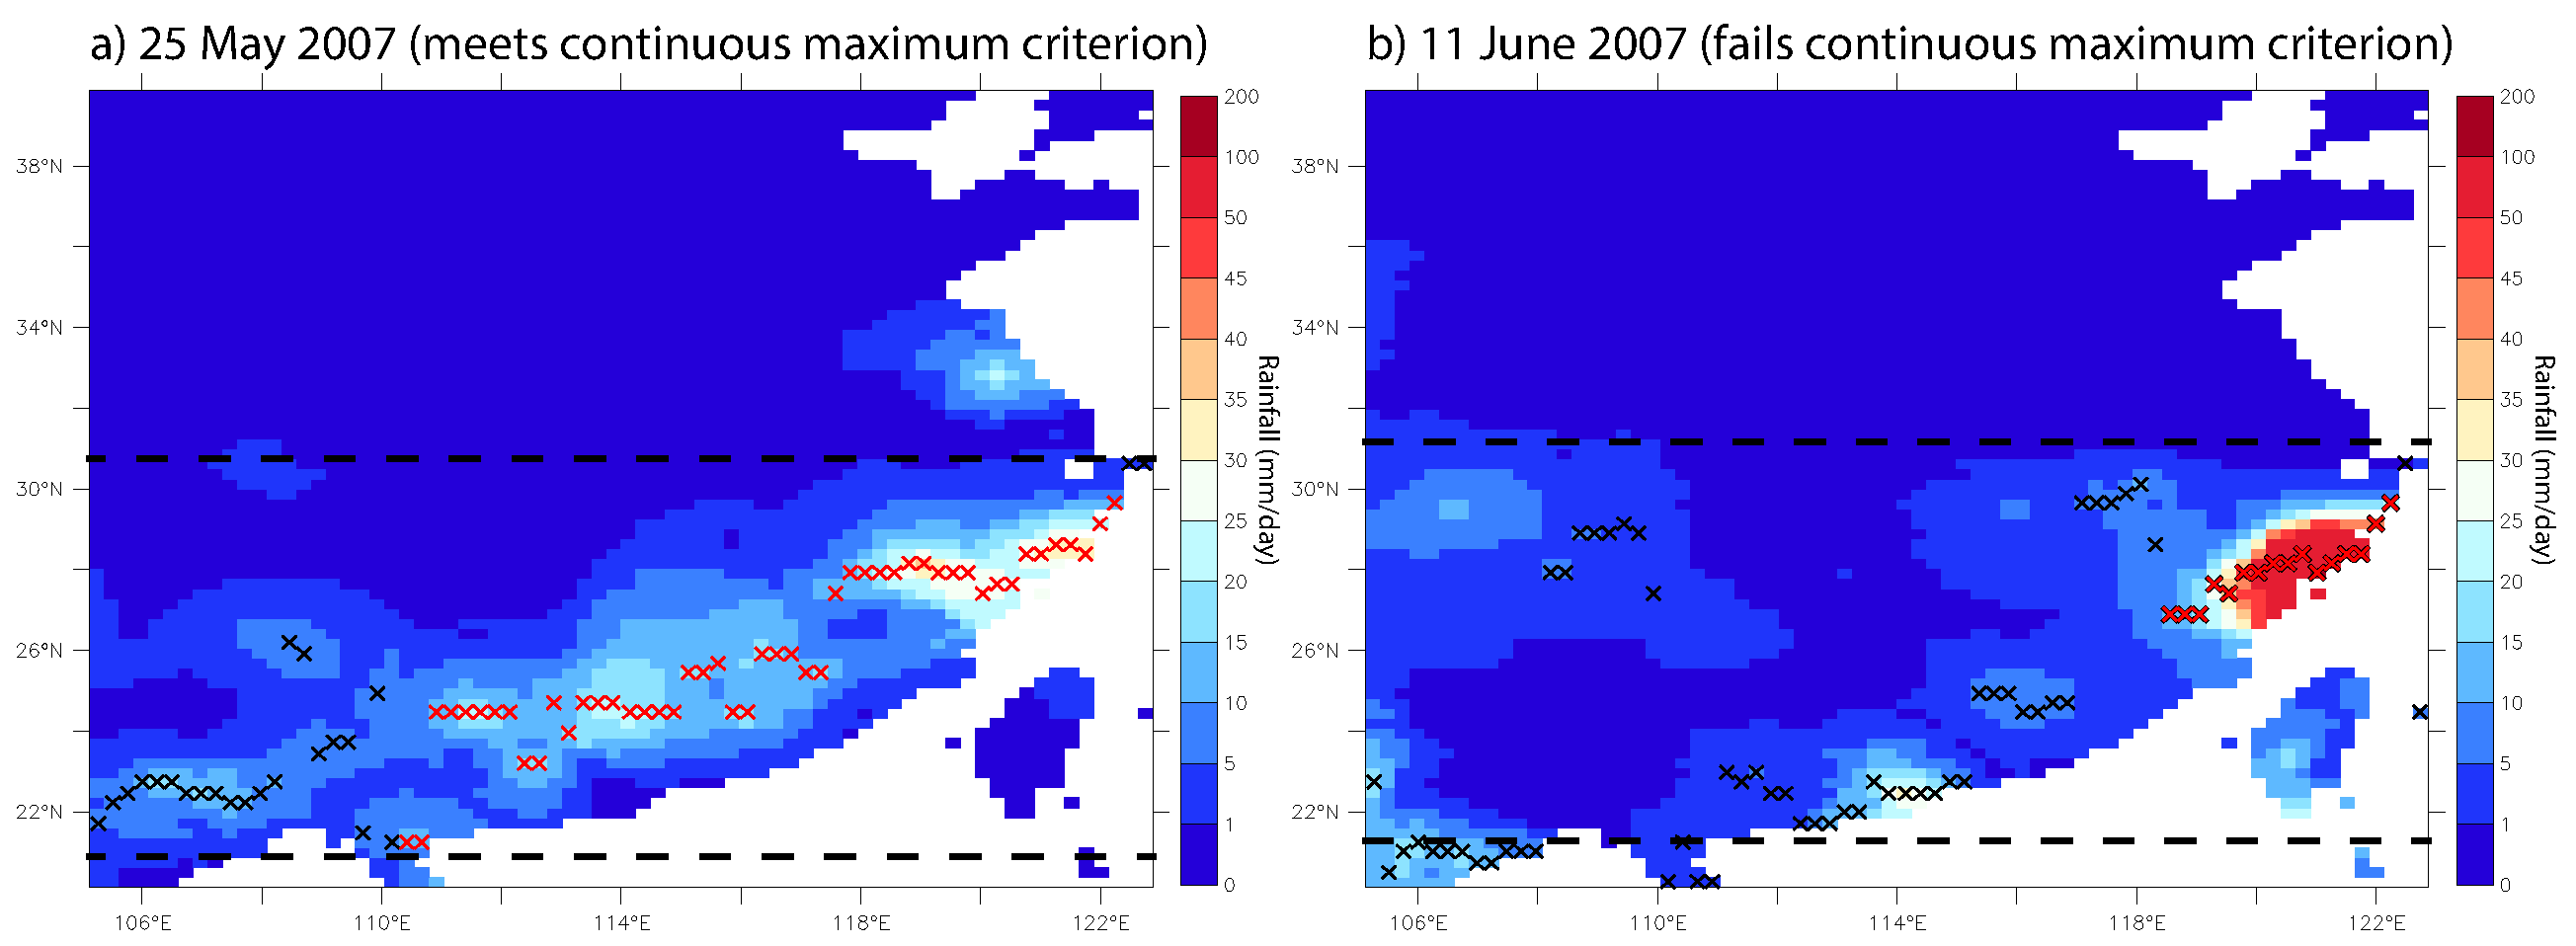
\includegraphics[width=40pc]{Figures/S1}
\caption{On each day, RDA first checks whether a continuous band of precipitation maxima exceeding 10 mm day$^{-1}$ exists that spans over 5 degrees of longitude. If so, a rainband fit is attempted. In panels a and b, the latitude of maximum precipitation at each longitude is marked with a black X. The longest continuous chain of maxima exceeding 10 mm day$^{-1}$ is marked in red. a) 25 May 2007 - the continuous maximum criterion is met and a fit is attempted.  b) 11 June 2007 - although there is abundant rainfall in some locations, no band is visible and the continuous maximum criterion is failed. No fit is attempted.}
\label{fig:f32}
\end{figure}

%%FIGURE 2 - How the convergent fit algorithm works.
\begin{figure}[htbp]
\centering
\noindent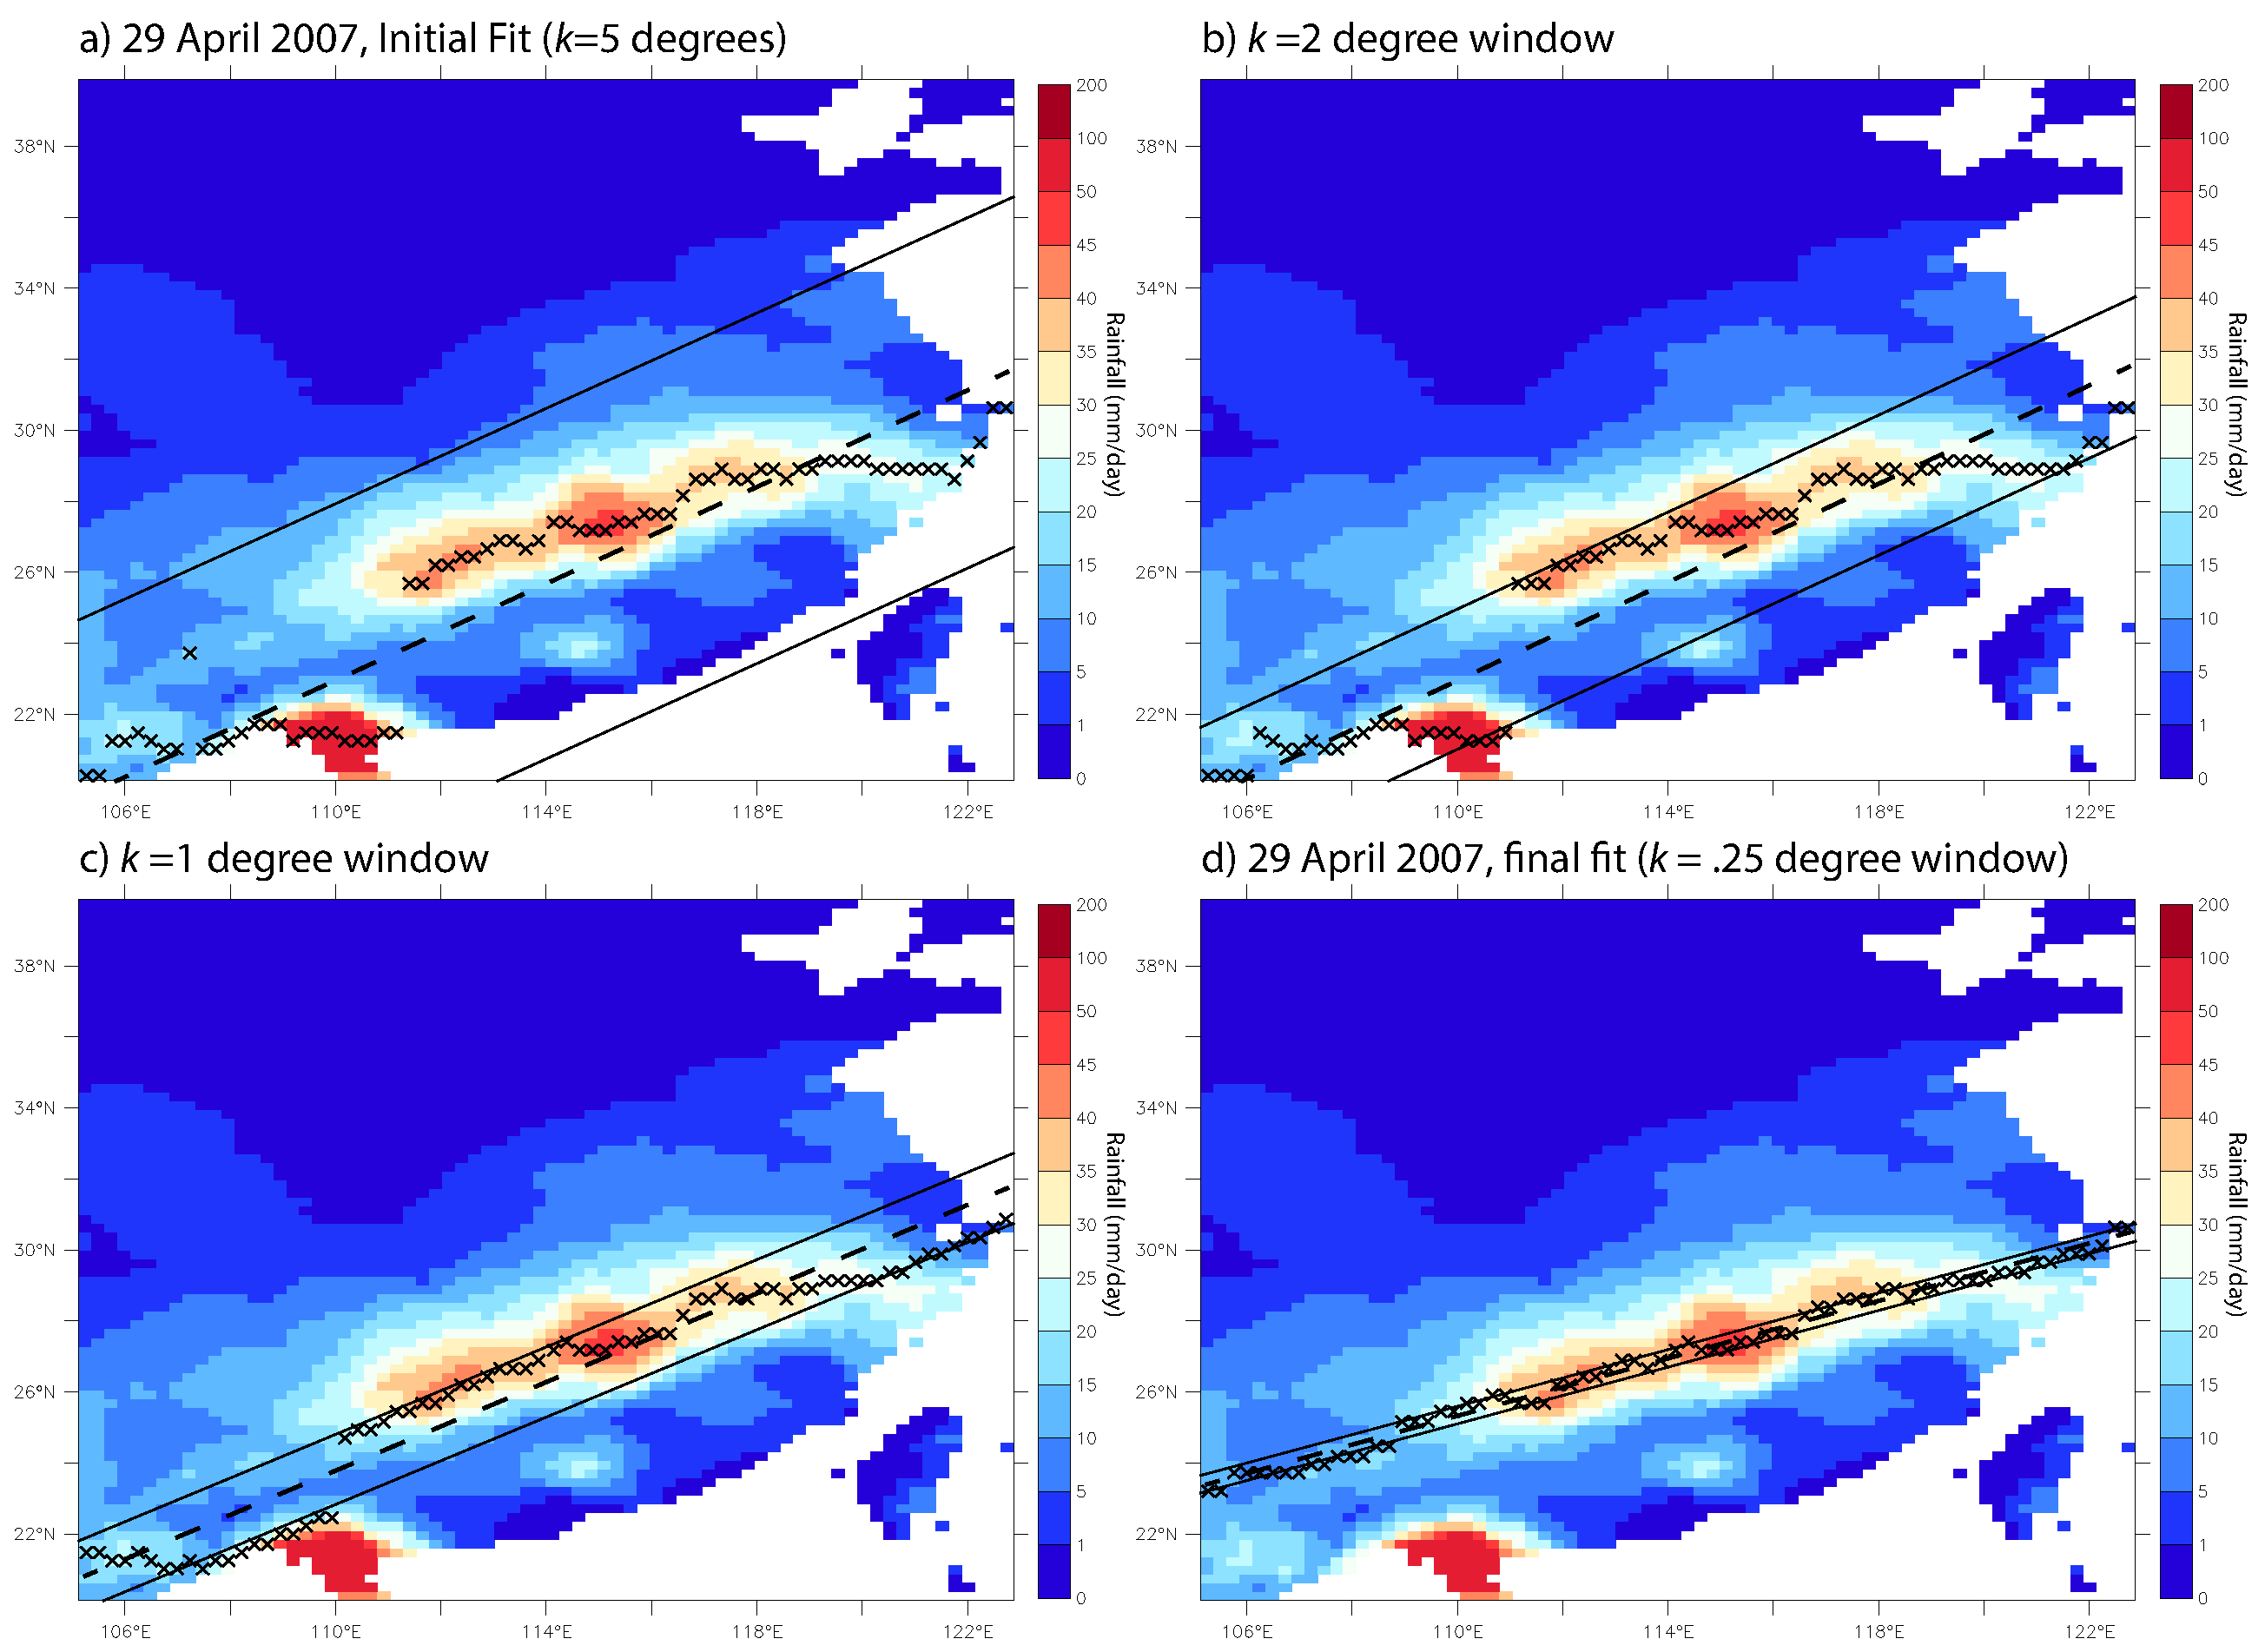
\includegraphics[width=40pc]{Figures/S2}
\caption{Display of the functionality of the recursive convergent fit. Dashed line shows estimated rainband position before each iteration and the solid lines indicate the window within we search for maxima. On 29 April 2007, a strong maximum in southernmost China skews our initial rainband fit (a), but the algorithm eventually converges on its true position via tighter windowing (d).}
\label{fig:f33}
\end{figure}

\clearpage

%%FIGURE 3 - Quality Control algorithm used to determine inclusion in statistics
\begin{figure}[htbp]
\centering
\noindent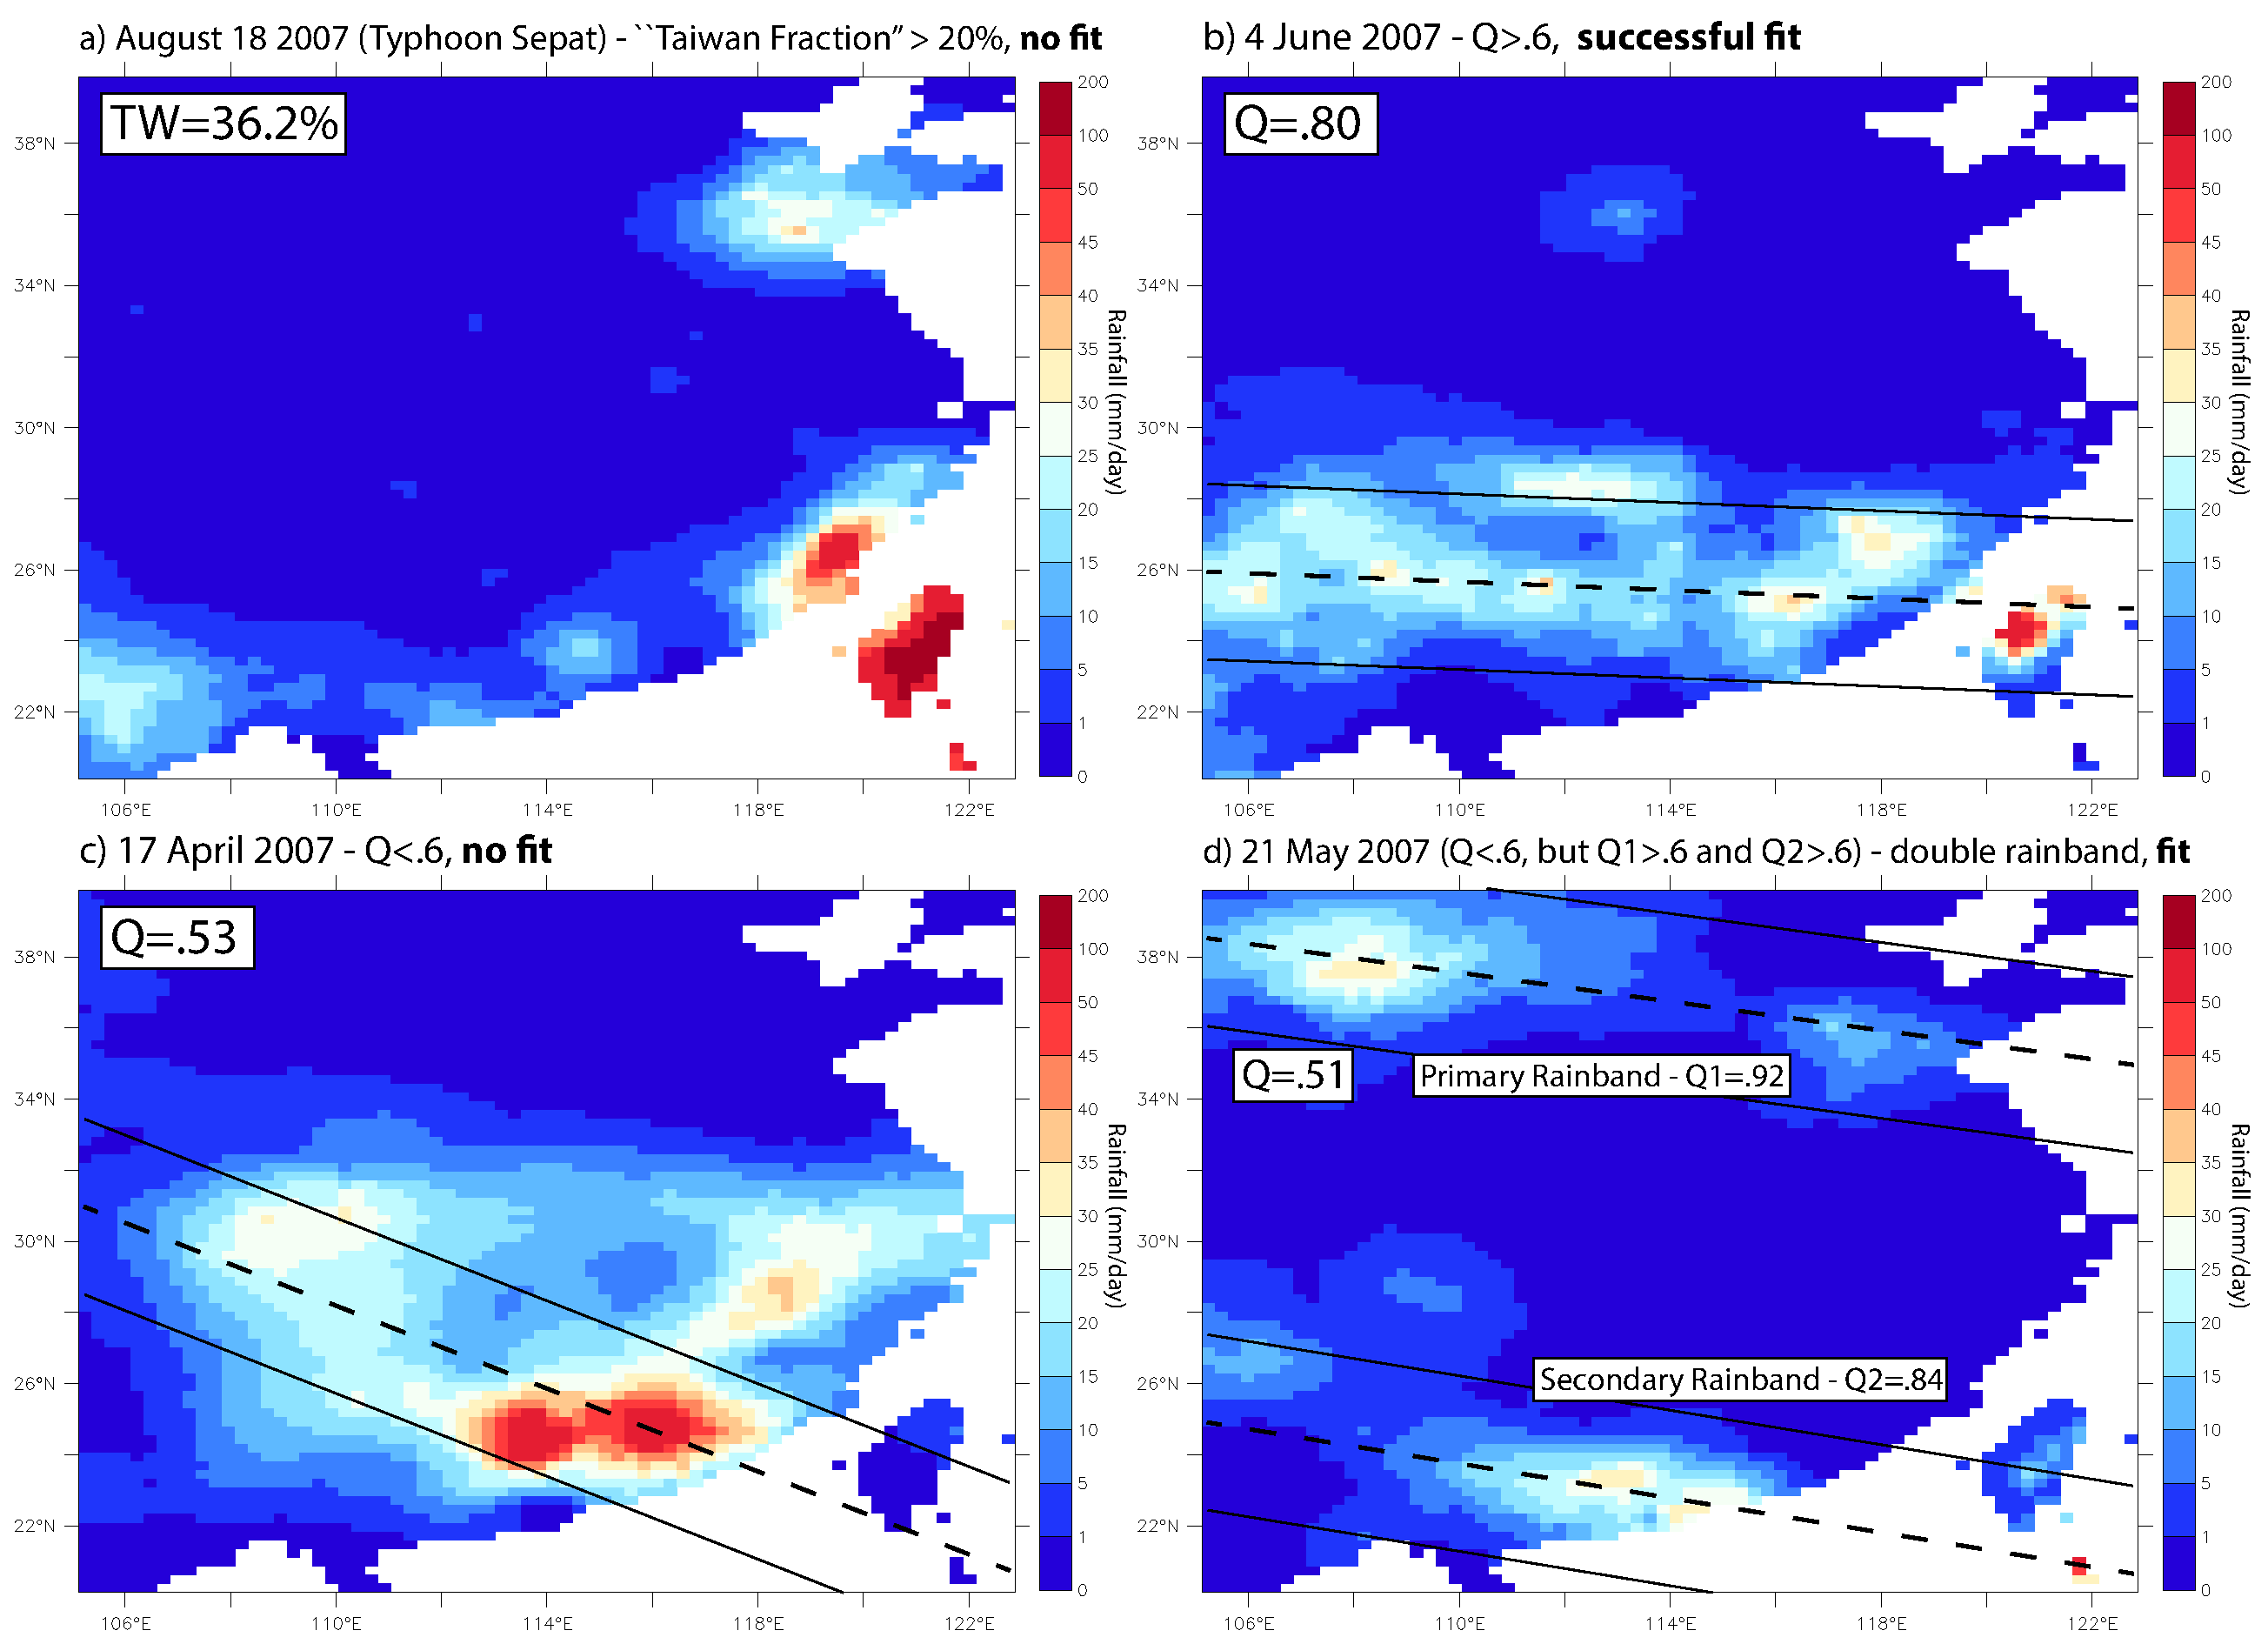
\includegraphics[width=40pc]{Figures/S4}
\caption{A quality control algorithm is used to exclude poor fits. a) 18 August 2007 - Days with a high Taiwan fraction (here, corresponding to the passage of Typhoon Sepat) are excluded from our statistics. b) June 4 2007 - A high-quality fit is achieved. c) 17 April 2007 - Although a tentative fit is obtained, it explains the distribution of rainfall poorly and is therefore unsuccessful. d) 21 May 2007 (same day as Figure~\ref{fig:f35}) - An initial fit appears to be of poor quality ($Q<.6$). However, after finding a secondary rainband, we determine that conditional quality scores $Q_1$ and $Q_2$ are sufficiently high, and the double rainband fit is successful.}
\label{fig:f34}
\end{figure}

%%FIGURE 4 - Procedure for finding double rainbands
\begin{figure}[htbp]
\centering
\noindent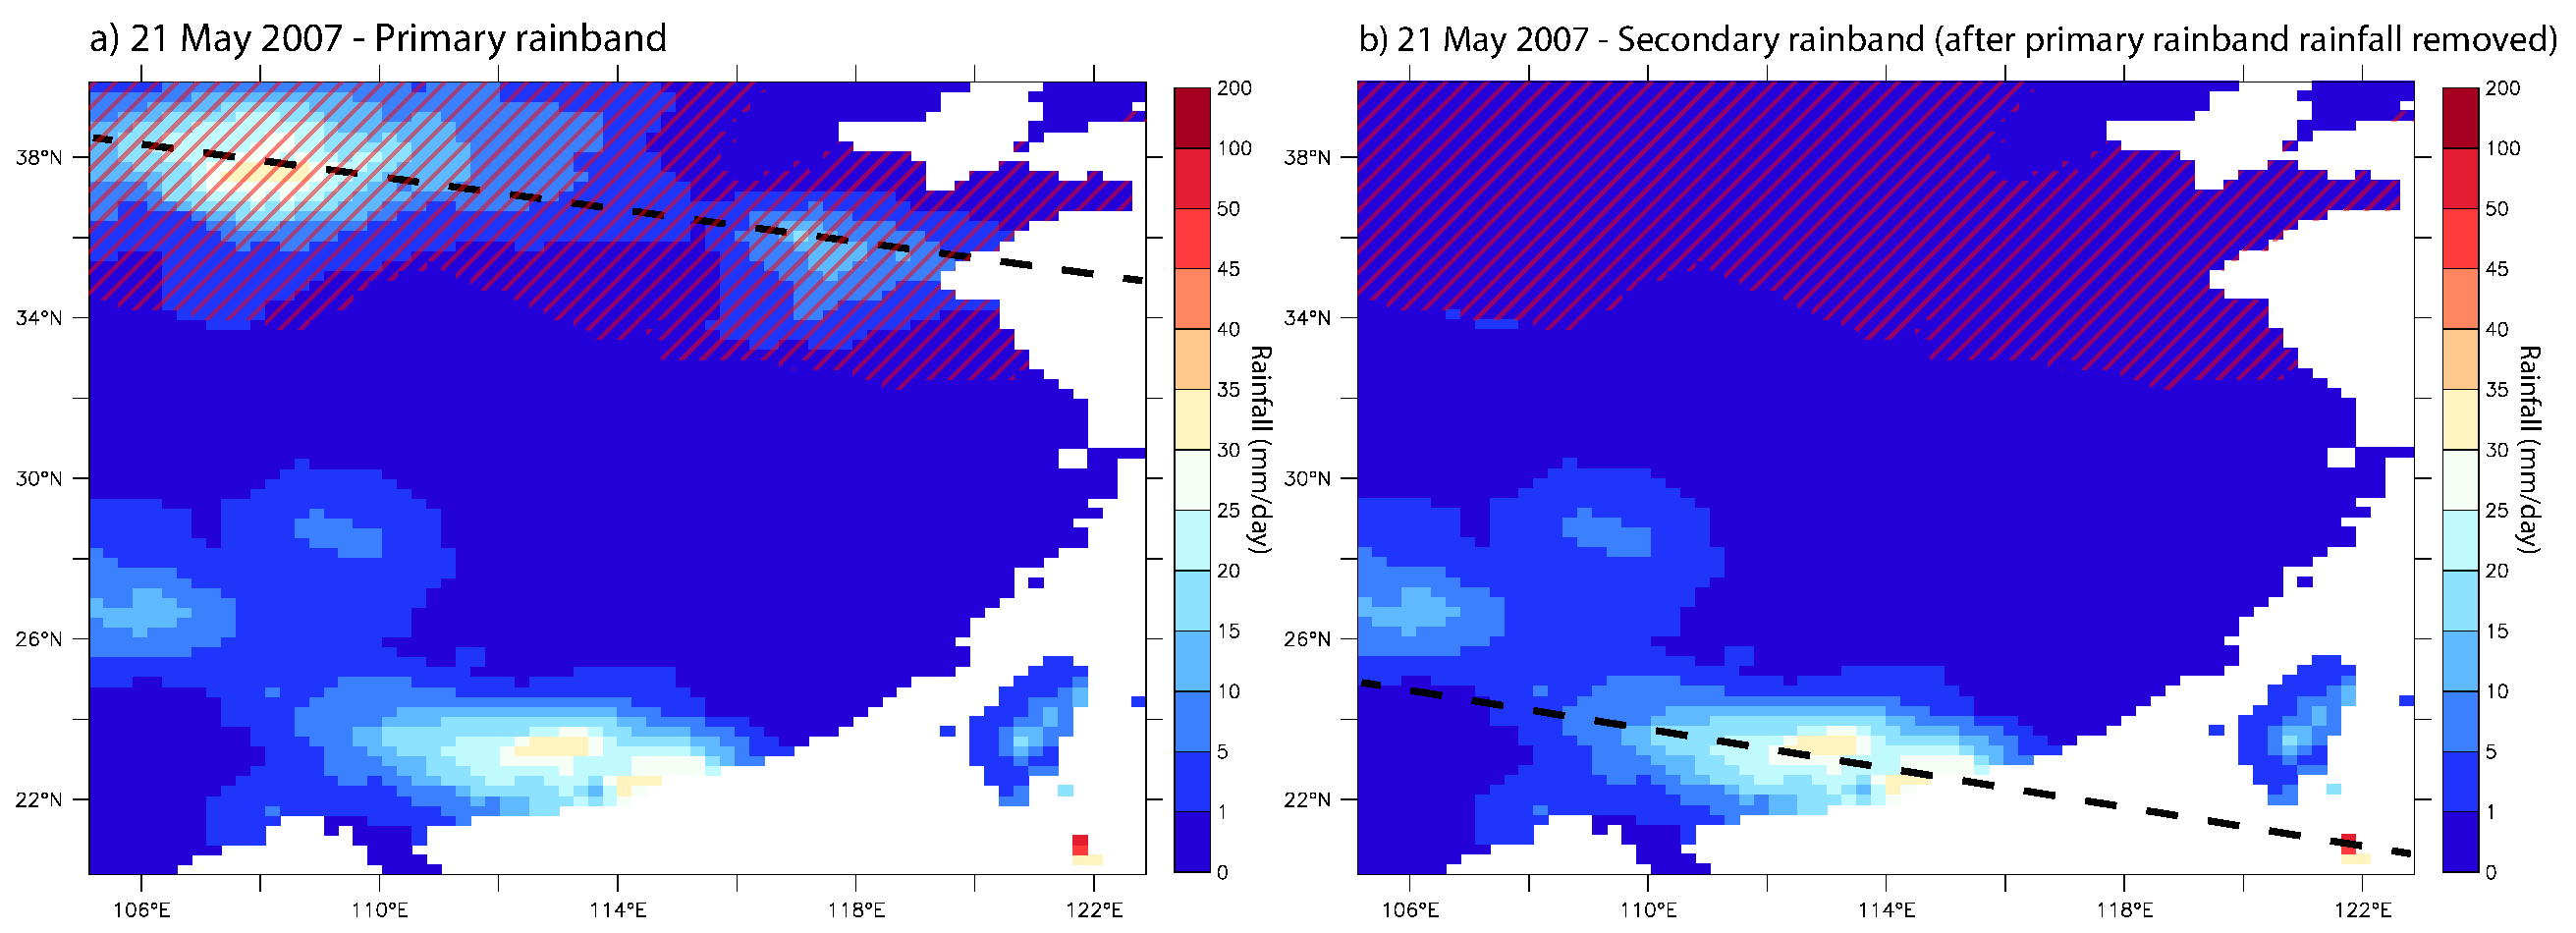
\includegraphics[width=42pc]{Figures/S3}
\caption{a) The first pass of the recursive fit algorithm converges on the strongest rainband, around 37$^{\circ}$N (defined as the ``primary rainband''). The \textit{banded rainfall} associated with the primary band is shaded with red hatchmarks. b) All banded rainfall from the primary band is removed, and we check for the presence of another rainband (a ``secondary rainband''), again using the continuous maximum criterion. When this criterion is satisfied, we find the secondary rainband's position with the recursive fit algorithm.}
\label{fig:f35}
\end{figure}

\clearpage

% FIGURES SHOWING RESULTS %%

%%FIGURE 5 Hovm�ller diagram of Meiyu latitude occupancy, 1951-2007. Produced by MATLAB scripts meiyufig1.m and meiyustats_compact.m.
\begin{figure}[htbp]
\centering
\noindent\includegraphics[width=32pc]{Figures/meiyu_hovmoller}
\caption{Climatology of East Asian rainfall and rainbands, 1951-2007, with important time periods marked as follows: 1 - Spring Rains; 2 - Pre-Meiyu; 3 - Meiyu; 4 - Post-Meiyu; 5 - Fall Rains. a) Hovm\"oller diagram of precipitation (100-123$^{\circ}$E longitudinal average); b) Hovm\"oller diagram of absolute probability of observing a rainband (both primary and secondary), smoothed in time with a 9-day and 2$^{\circ}$-running box filter; c) Probability of primary rainband occurrence and mean intensity (9-day running mean); d) The conditional probability of a secondary rainband given the presence of a primary rainband, as well as the mean tilt and length of primary rainband events (9-day running mean).}
\label{fig:hov}
\end{figure}

%%FIGURE 6 Percentage of total rainfall at each point that is delivered through rainbands
%% CAN I DO A SEASONAL VERSION OF THIS FILE?!
\begin{figure}[htb]
\centering
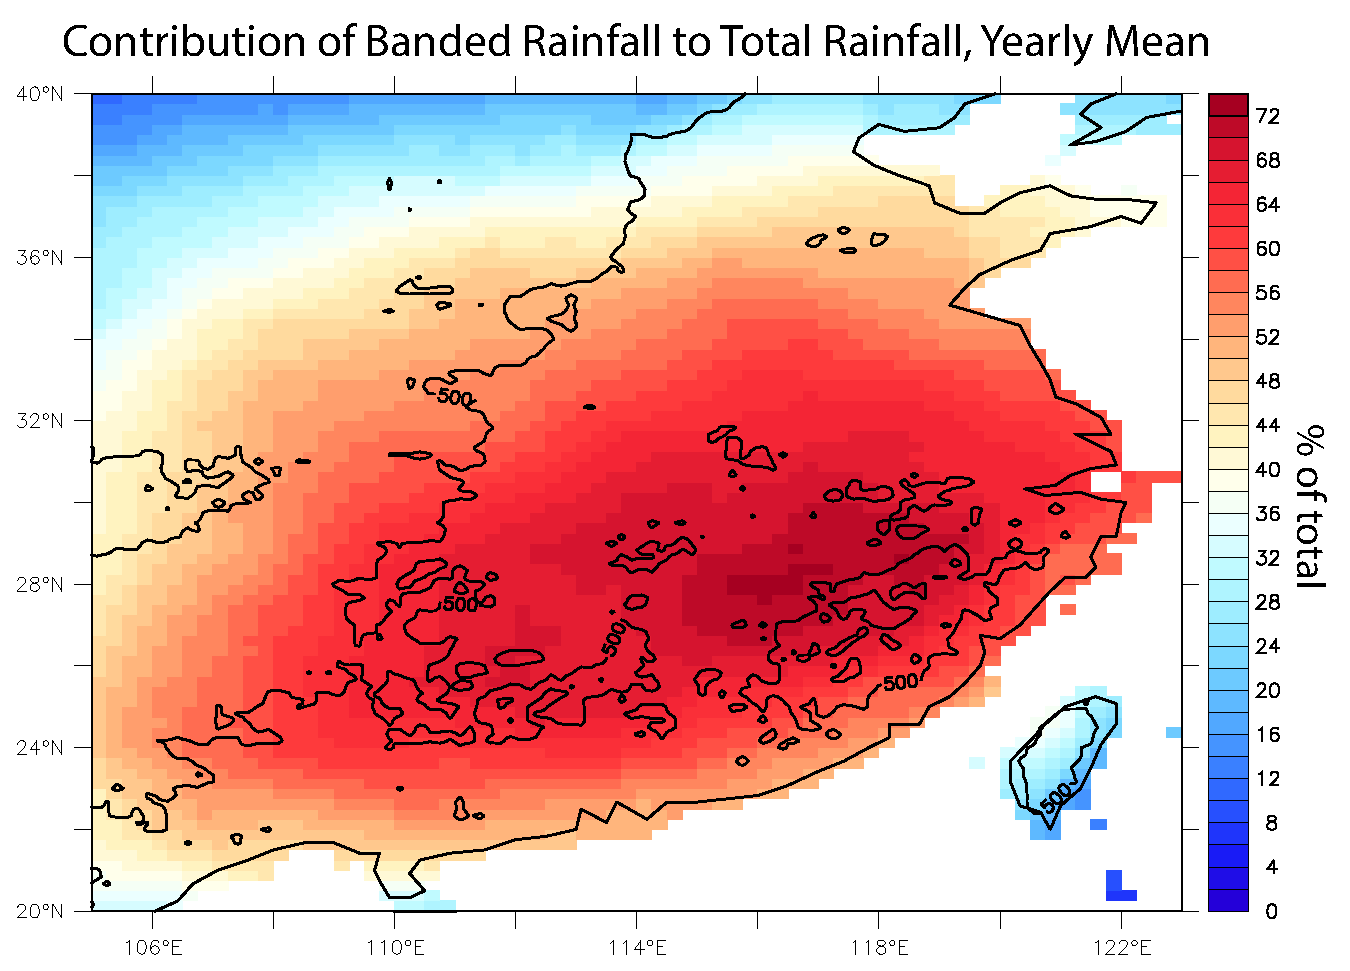
\includegraphics[width=36pc]{Figures/frontpct_topo}
\caption{Yearly mean percentage of total rainfall that falls as banded rainfall. On a given day, banded rainfall consists of all rainfall falling within 4$^{\circ}$ of a rainband axis and rainfall at any other adjacent point exceeding 10 mm day$^{-1}$.}
\label{fig:frontpct}
\end{figure}

%%FIGURE 7 - the South Flood-North Drought shown in a single figure.
\begin{figure}
\centering
\noindent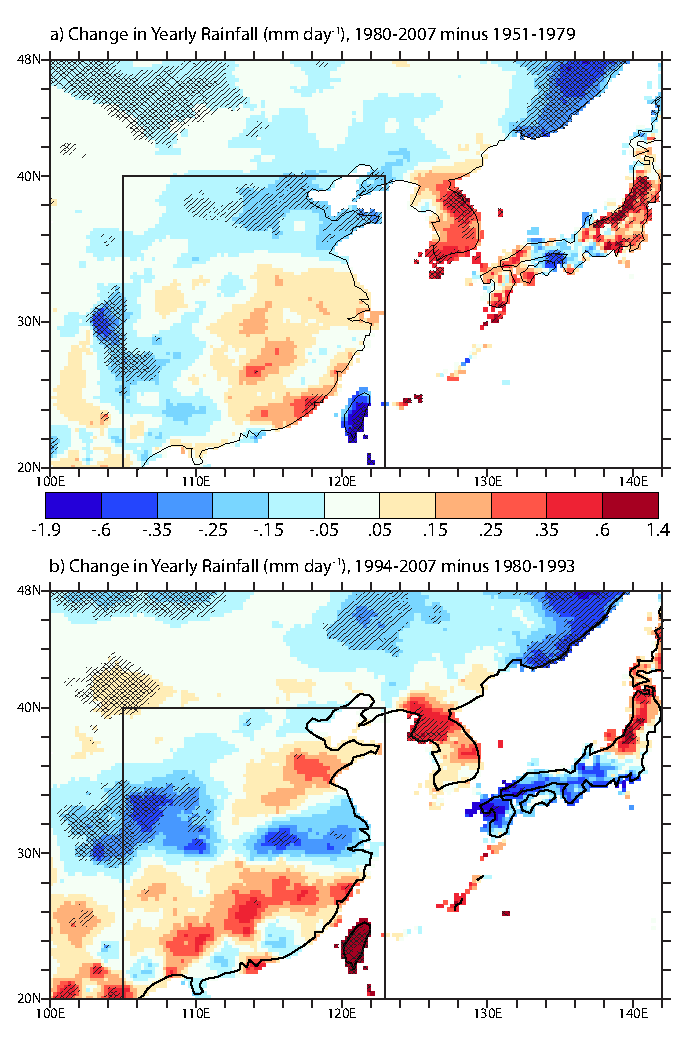
\includegraphics[width=36pc]{Figures/SFND}
\caption{Difference in East Asian yearly mean rainfall for 1980-2007 relative to a baseline of 1951-1979. The region of application of RDA spans 105-123$^{\circ}$E and 20-40$^{\circ}$N over eastern China and Taiwan (marked by box). Changes significant at a 95\%/99\% level are marked with single/double cross-hatches respectively as calculated by permutation test with 1,000 iterations.}
\label{fig:sfnd}
\end{figure}

%%FIGURE 8 Changes in Meiyu and rainfall behavior between 1951-1979 and 1980-2007
\begin{figure}[htbp]
\centering
\noindent\includegraphics[width=36pc]{Figures/changes}
\caption{a) 15-day running mean of the change in rainfall between 1951-1979 and 1980-07, with 95\%/99\% confidence level marked by single/double cross-hatches; b) 15-day running mean of the change in rainband frequency between 1951-1979 and 1980-07, with two-degree smoothing in latitude and confidence levels marked as in a). The significance of rainfall changes is calculated by a permutation method. Time periods are marked as in Figure~\ref{fig:hov}: 1 - Spring Rains; 2 - Pre-Meiyu; 3 - Meiyu; 4 - Post-Meiyu; 5 - Fall Rains.}
\label{fig:changes}
\end{figure}

%%FIGURE 9 Climatology of alternative metrics of China rainfall
\begin{figure}[htb]
\centering
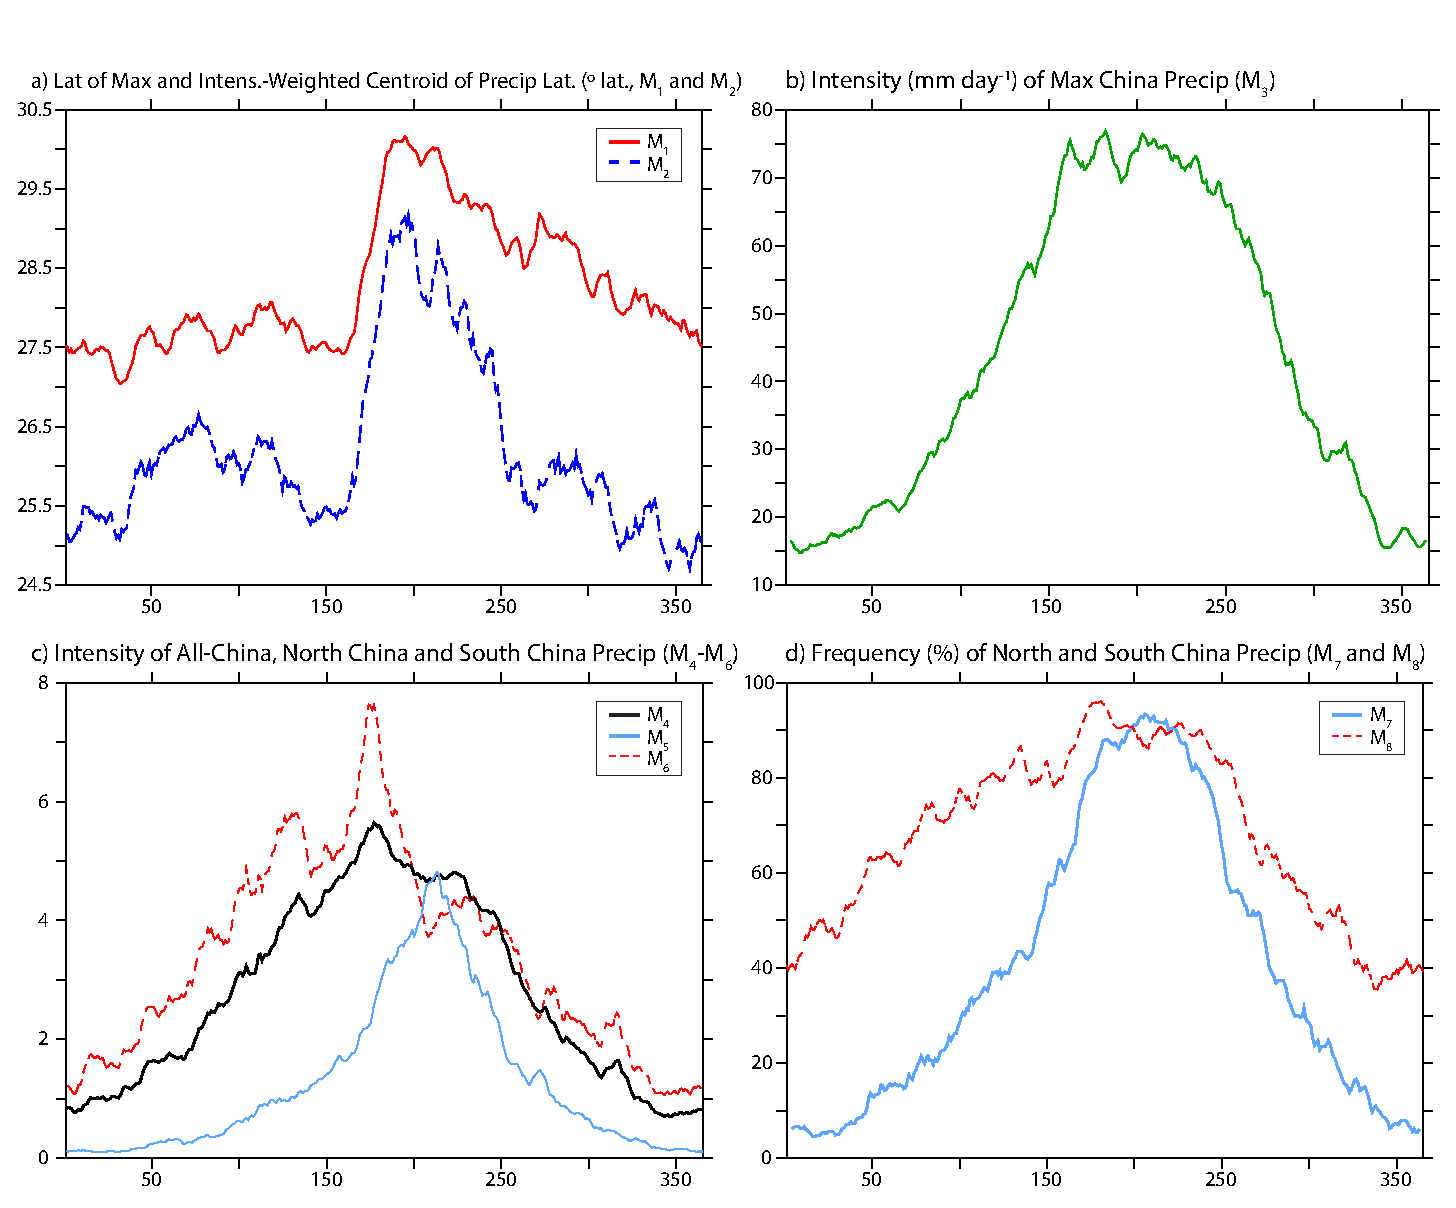
\includegraphics[width=36pc]{Figures/met_climo}
\caption{Yearly climatology of alternative metrics of China rainfall $M_1-M_8$. a) Latitude of maximum precipitation (blue dash, $M_1$) and intensity-weighted centroid of precipitation latitude (red, $M_2$); b) Intensity of maximum precipitation over China ($M_3$); c) Mean intensity of China rainfall (black, $M_4$), North China rainfall (thin light blue, $M_5$) and South China rainfall (red dash, $M_6$); d) Frequency of North China rainfall (light blue, $M_7$) and South China rainfall (red, $M_8$). China region is defined as 105-123$^{\circ}$E and 20-40$^{\circ}$N, North China as 107.5-125$^{\circ}$E and 37-42$^{\circ}$N and South China as 107.5-122.5$^{\circ}$E and 27-33$^{\circ}$N.}
\label{fig:met_climo}
\end{figure}

%%FIGURE 10 Decadal mean in different rainfall types during different time periods
\begin{figure}[htb]
\centering
\noindent\includegraphics[width=38pc]{Figures/RDA_type_climo_topo}
\caption{Climatology of the amount of total rainfall, banded rainfall and local rainfall for the full year, Pre-Meiyu (days 121-160), Meiyu (days 161-200) and Post-Meiyu (days 201-273). \textit{Banded} rainfall consists of all rainfall falling within 4$^{\circ}$ of a rainband axis and rainfall at any other adjacent point exceeding 10 mm day$^{-1}$. \textit{Local} rainfall includes all rainfall not meeting these criteria.}
\label{fig:type_climo}
\end{figure}

%%FIGURE 11 Decadal changes in different rainfall types
%potential change - add the total change in rainfall for each of the time periods (third column of panels)
\begin{figure}[htb]
\centering
\noindent\includegraphics[width=38pc]{Figures/RDA_type_decadal}
\caption{1980-2007 versus 1951-1979 changes in total, banded and local rainfall for full year, Pre-Meiyu (days 121-160), Meiyu (days 161-200) and Post-Meiyu (days 201-273), with significance at the 95\%/99\% level marked by single/double hatches (permutation test with 1,000 iterations). \textit{Banded} rainfall consists of all rainfall falling within 4$^{\circ}$ of a rainband axis and rainfall at any other adjacent point exceeding 10 mm day$^{-1}$. \textit{Local} rainfall includes all rainfall not meeting these criteria.}
\label{fig:type_decadal}
\end{figure}


\end{document}